\documentclass{article}
% \usepackage[utf8]{inputenc}

% FONTS
\usepackage[T1]{fontenc}
\usepackage{tgtermes}
\usepackage{amsmath}

% Font choice 2:
\usepackage[scaled=0.92]{PTSans}
\usepackage{amssymb}
\newcommand{\mathbold}[1]{\ensuremath{\boldsymbol{\mathbf{#1}}}}
\newcommand{\mbf}[1]{\ensuremath{\boldsymbol{\mathbf{#1}}}}

% \usepackage{lmodern}

%\usefonttheme{professionalfonts}

\usepackage{scalefnt,letltxmacro}
\LetLtxMacro{\oldtextsc}{\textsc}
\renewcommand{\textsc}[1]{\oldtextsc{\fontfamily{lmr}\scalefont{1}#1}}

% \renewcommand*\ttdefault{lmvtt}
\usepackage[ttdefault=true]{AnonymousPro}

% GEOMETRY
%\usepackage[
%  paper  = letterpaper,
%  left   = 1.65in,
%  right  = 1.65in,
%  top    = 1.0in,
%  bottom = 1.0in,
%  ]{geometry}

% # COLOR

% \usepackage[usenames,dvipsnames]{xcolor}
\definecolor{shadecolor}{gray}{0.9}

% \newcommand{\red}[1]{\textcolor{BrickRed}{#1}}
% \newcommand{\orange}[1]{\textcolor{BurntOrange}{#1}}
% \newcommand{\green}[1]{\textcolor{OliveGreen}{#1}}
% \newcommand{\blue}[1]{\textcolor{MidnightBlue}{#1}}
% \newcommand{\sky}[1]{\textcolor{SkyBlue}{#1}}
% \newcommand{\gray}[1]{\textcolor{black!60}{#1}}

% SPACING and TEXT
%\usepackage[final,expansion=alltext]{microtype}
\usepackage[english]{babel}
\usepackage[parfill]{parskip}
\usepackage{afterpage}
\usepackage{framed}
\usepackage{xspace}

% LEFTBAR
\renewenvironment{leftbar}[1][\hsize]
{%
  \def\FrameCommand
  {%
    {\color{Gray}\vrule width 3pt}%
    \hspace{10pt}%
    %\hspace{0pt}\fboxsep=\FrameSep\colorbox{black!10}%
  }%
  \MakeFramed{\hsize#1\advance\hsize-\width\FrameRestore}%
}%
{\endMakeFramed}

% EDITING
% line numbering in left margin
\usepackage{lineno}
\renewcommand\linenumberfont{\normalfont
                             \footnotesize
                             \sffamily
                             \color{SkyBlue}}
% ragged paragraphs in right margin
\usepackage{ragged2e}
% TODO should i rename sidenote marginpar?
\DeclareRobustCommand{\sidenote}[1]{\marginpar{
                                    \RaggedRight
                                    \textcolor{Plum}{\textsf{#1}}}}
% paragraph counter in right margin
\newcommand{\parnum}{\bfseries\P\arabic{parcount}}
\newcounter{parcount}
\newcommand\p{%
    \stepcounter{parcount}%
    \leavevmode\marginpar[\hfill\parnum]{\parnum}%
}
% pargraph header
\DeclareRobustCommand{\parhead}[1]{\textbf{#1}~}
% paragraph helper
\DeclareRobustCommand{\PP}{\textcolor{Plum}{\P} }

% COUNTERS
%\renewcommand{\labelenumi}{\color{black!67}{\arabic{enumi}.}}
%\renewcommand{\labelenumii}{{\color{black!67}(\alph{enumii})}}
%\renewcommand{\labelitemi}{{\color{black!67}\textbullet}}

% FIGURES
\usepackage{graphicx}
\usepackage[labelfont=bf]{caption}
%\usepackage[format=hang]{subcaption}

% TABLES
\usepackage{booktabs}

% # ALGORITHMS

\usepackage[algoruled]{algorithm2e}
\setlength{\interspacetitleruled}{8pt}
\usepackage{listings}
\usepackage{fancyvrb}
\fvset{fontsize=\small}

% HYPERREF
%\usepackage[colorlinks,linktoc=all]{hyperref}
%\usepackage[all]{hypcap}
\hypersetup{citecolor=Plum}
\hypersetup{linkcolor=MidnightBlue}
\hypersetup{urlcolor=MidnightBlue}

% CLEVEREF must come after HYPERREF
\usepackage[nameinlink]{cleveref}
\newcommand{\Crefb}[1]{(\Cref{#1})}
\newcommand{\crefb}[1]{(\cref{#1})}

% ACRONYMS
\usepackage[acronym,smallcaps,nowarn]{glossaries}
\glsdisablehyper
% \makeglossaries

% COLOR DEFINITIONS
\newcommand{\red}[1]{\textcolor{BrickRed}{#1}}
\newcommand{\orange}[1]{\textcolor{BurntOrange}{#1}}
\newcommand{\green}[1]{\textcolor{OliveGreen}{#1}}
\newcommand{\blue}[1]{\textcolor{MidnightBlue}{#1}}
\newcommand{\gray}[1]{\textcolor{black!60}{#1}}

% CODE
\usepackage{minted}  % for syntax highlighting

% REFERENCES
\usepackage[
  backend=biber,
  natbib,
  doi=false,isbn=false,url=false,
  sorting=none,
  citestyle=authoryear]{biblatex}

\newacronym{PPL}{ppl}{probabilistic programming language}
\newacronym{GPU}{\textnormal{\uppercase{gpu}}}{graphics processing unit}

\newacronym{VAE}{vae}{variational auto-encoder}
\newacronym{RBM}{rbm}{restricted Boltzmann machine}
\newacronym{DLGM}{dlgm}{deep latent Gaussian model}
\newacronym{GAN}{gan}{generative adversarial network}
\newacronym{RNN}{rnn}{recurrent neural network}

\newacronym{VI}{vi}{variational inference}
\newacronym{MCMC}{mcmc}{Markov chain Monte Carlo}
\newacronym{MC}{mc}{Monte Carlo}
\newacronym{HMC}{hmc}{Hamiltonian Monte Carlo}
\newacronym{MAP}{map}{maximum a posteriori}
\newacronym{IWAE}{iwae}{importance-weighted auto-encoder}
\newacronym{HVM}{hvm}{hierarchical variational model}
\newacronym{KL}{kl}{Kullback-Leibler}
\newacronym{ELBO}{elbo}{\emph{evidence lower bound}}

\DeclareRobustCommand{\mb}[1]{\ensuremath{\boldsymbol{\mathbf{#1}}}}

\newcommand{\mba}{\mathbold{a}}
\newcommand{\mbb}{\mathbold{b}}
\newcommand{\mbc}{\mathbold{c}}
\newcommand{\mbd}{\mathbold{d}}
\newcommand{\mbe}{\mathbold{e}}
%\newcommand{\mbf}{\mathbold{f}}
\newcommand{\mbg}{\mathbold{g}}
\newcommand{\mbh}{\mathbold{h}}
\newcommand{\mbi}{\mathbold{i}}
\newcommand{\mbj}{\mathbold{j}}
\newcommand{\mbk}{\mathbold{k}}
\newcommand{\mbl}{\mathbold{l}}
\newcommand{\mbm}{\mathbold{m}}
\newcommand{\mbn}{\mathbold{n}}
\newcommand{\mbo}{\mathbold{o}}
\newcommand{\mbp}{\mathbold{p}}
\newcommand{\mbq}{\mathbold{q}}
\newcommand{\mbr}{\mathbold{r}}
\newcommand{\mbs}{\mathbold{s}}
\newcommand{\mbt}{\mathbold{t}}
\newcommand{\mbu}{\mathbold{u}}
\newcommand{\mbv}{\mathbold{v}}
\newcommand{\mbw}{\mathbold{w}}
\newcommand{\mbx}{\mathbold{x}}
\newcommand{\mby}{\mathbold{y}}
\newcommand{\mbz}{\mathbold{z}}

\newcommand{\mbA}{\mathbold{A}}
\newcommand{\mbB}{\mathbold{B}}
\newcommand{\mbC}{\mathbold{C}}
\newcommand{\mbD}{\mathbold{D}}
\newcommand{\mbE}{\mathbold{E}}
\newcommand{\mbF}{\mathbold{F}}
\newcommand{\mbG}{\mathbold{G}}
\newcommand{\mbH}{\mathbold{H}}
\newcommand{\mbI}{\mathbold{I}}
\newcommand{\mbJ}{\mathbold{J}}
\newcommand{\mbK}{\mathbold{K}}
\newcommand{\mbL}{\mathbold{L}}
\newcommand{\mbM}{\mathbold{M}}
\newcommand{\mbN}{\mathbold{N}}
\newcommand{\mbO}{\mathbold{O}}
\newcommand{\mbP}{\mathbold{P}}
\newcommand{\mbQ}{\mathbold{Q}}
\newcommand{\mbR}{\mathbold{R}}
\newcommand{\mbS}{\mathbold{S}}
\newcommand{\mbT}{\mathbold{T}}
\newcommand{\mbU}{\mathbold{U}}
\newcommand{\mbV}{\mathbold{V}}
\newcommand{\mbW}{\mathbold{W}}
\newcommand{\mbX}{\mathbold{X}}
\newcommand{\mbY}{\mathbold{Y}}
\newcommand{\mbZ}{\mathbold{Z}}

\newcommand{\mbalpha}{\mathbold{\alpha}}
\newcommand{\mbbeta}{\mathbold{\beta}}
\newcommand{\mbdelta}{\mathbold{\delta}}
\newcommand{\mbepsilon}{\mathbold{\epsilon}}
\newcommand{\mbchi}{\mathbold{\chi}}
\newcommand{\mbeta}{\mathbold{\eta}}
\newcommand{\mbgamma}{\mathbold{\gamma}}
\newcommand{\mbiota}{\mathbold{\iota}}
\newcommand{\mbkappa}{\mathbold{\kappa}}
\newcommand{\mblambda}{\mathbold{\lambda}}
\newcommand{\mbmu}{\mathbold{\mu}}
\newcommand{\mbnu}{\mathbold{\nu}}
\newcommand{\mbomega}{\mathbold{\omega}}
\newcommand{\mbphi}{\mathbold{\phi}}
\newcommand{\mbpi}{\mathbold{\pi}}
\newcommand{\mbpsi}{\mathbold{\psi}}
\newcommand{\mbrho}{\mathbold{\rho}}
\newcommand{\mbsigma}{\mathbold{\sigma}}
\newcommand{\mbtau}{\mathbold{\tau}}
\newcommand{\mbtheta}{\mathbold{\theta}}
\newcommand{\mbupsilon}{\mathbold{\upsilon}}
\newcommand{\mbvarepsilon}{\mathbold{\varepsilon}}
\newcommand{\mbvarphi}{\mathbold{\varphi}}
\newcommand{\mbvartheta}{\mathbold{\vartheta}}
\newcommand{\mbvarrho}{\mathbold{\varrho}}
\newcommand{\mbxi}{\mathbold{\xi}}
\newcommand{\mbzeta}{\mathbold{\zeta}}

\newcommand{\mbDelta}{\mathbold{\Delta}}
\newcommand{\mbGamma}{\mathbold{\Gamma}}
\newcommand{\mbLambda}{\mathbold{\Lambda}}
\newcommand{\mbOmega}{\mathbold{\Omega}}
\newcommand{\mbPhi}{\mathbold{\Phi}}
\newcommand{\mbPi}{\mathbold{\Pi}}
\newcommand{\mbPsi}{\mathbold{\Psi}}
\newcommand{\mbSigma}{\mathbold{\Sigma}}
\newcommand{\mbTheta}{\mathbold{\Theta}}
\newcommand{\mbUpsilon}{\mathbold{\Upsilon}}
\newcommand{\mbXi}{\mathbold{\Xi}}

\renewcommand{\d}[1]{\ensuremath{\operatorname{d}\!{#1}}}
\newcommand{\g}{\,|\,}
\renewcommand{\gg}{\,\|\,}
\newcommand\dif{\mathop{}\!\mathrm{d}}
\newcommand{\diag}{\textrm{diag}}
\newcommand{\supp}{\textrm{supp}}
\newcommand{\Gam}{\textrm{Gam}}
\newcommand{\InvGam}{\textrm{InvGam}}
\DeclareMathOperator*{\argmax}{arg\,max}
\DeclareMathOperator*{\argmin}{arg\,min}
\DeclareRobustCommand{\KL}[2]{\ensuremath{\textrm{KL}\left(#1\;\|\;#2\right)}}
\newcommand\indep{\protect\mathpalette{\protect\independenT}{\perp}}
\def\independenT#1#2{\mathrel{\rlap{$#1#2$}\mkern2mu{#1#2}}}
\newcommand{\E}[1]{\mathbb{E}\left[ #1 \right]}

\usepackage{tikz}
\usetikzlibrary{bayesnet}

\pgfdeclarelayer{edgelayer}
\pgfdeclarelayer{nodelayer}
\pgfsetlayers{edgelayer,nodelayer,main}

\definecolor{hexcolor0xbfbfbf}{rgb}{0.749,0.749,0.749}

\tikzset{>=latex}
\tikzstyle{none}   = [inner sep=0pt]
\tikzstyle{line}   = [-,
                      thick,
                      shorten <=1pt,
                      shorten >=1pt]
\tikzstyle{arrow}  = [->,
                      thick,
                      shorten <=1pt,
                      shorten >=1pt]
\tikzstyle{ardash} = [dashed,
                      ->,
                      thick,
                      shorten <=1pt,
                      shorten >=1pt]

\tikzstyle{empty}=[
                   circle,
                   opacity=0.0,
                   text opacity=1.0,
                   inner sep=0pt
                  ]

\tikzstyle{box}=[
                 rectangle,
                 fill=White,
                 thick,
                 draw=Black,
                 inner sep=7pt
                ]

\tikzstyle{filled}=[
                    circle,
                    thick,
                    fill=hexcolor0xbfbfbf,
                    draw=Black
                   ]

\tikzstyle{hollow}=[
                    circle,
                    thick,
                    fill=White,
                    draw=Black
                   ]

\tikzstyle{param}=[
                   rectangle,
                   fill=Black,
                   draw=Black,
                   inner sep=0pt,
                   minimum width=4pt,
                   minimum height=4pt
                  ]

\tikzstyle{paramhollow}=[
                         rectangle,
                         thick,
                         fill=White,
                         draw=Black,
                         inner sep=0pt,
                         minimum
                         width=4pt,
                         minimum height=4pt
                        ]

\usepackage{pgfplots}                               % PGFPLOTS baby!
\pgfplotsset{compat=newest}
\pgfplotsset{plot coordinates/math parser=false}
% \usepgfplotslibrary{statistics}


\title{
Edward: A library for probabilistic modeling,\break inference, and criticism
}

\author{
Dustin Tran, Alp Kucukelbir, Adji B.~Dieng,\\
Maja Rudolph, Dawen Liang, and David M.~Blei\\\\
Columbia University
}

\begin{document}

\hypersetup{pageanchor=false}
\begin{titlepage}
\maketitle
\begin{abstract}
  Probabilistic modeling is a powerful approach for analyzing
  empirical information.
  We describe \emph{Edward}, a library for probabilistic modeling.
  Edward's design reflects an iterative process pioneered by George
  Box: build a model of a phenomenon, make inferences about the model given
  data, and criticize the model's fit to the data. Edward supports a broad class
  of probabilistic models, efficient algorithms for inference, and many
  techniques for model criticism. The library builds on top of
  TensorFlow to support distributed training and hardware such as
  GPUs.
  Edward enables the development of complex probabilistic
  models and their algorithms at a massive scale.
\end{abstract}

\emph{Keywords:}
Probabilistic Models;
Bayesian Inference;
Model Criticism;
Neural Networks;
Scalable Computation;
Probabilistic Programming.%
\footnote{Details in this paper describe Edward version 1.2.1,
released Jan 30, 2017.}

\setcounter{secnumdepth}{2}
\setcounter{tocdepth}{2}
\tableofcontents

\thispagestyle{empty}
\end{titlepage}
\hypersetup{pageanchor=true}

\glsresetall{}

\clearpage

\section{Introduction}
\label{sec:intro}

Probabilistic modeling is a powerful approach for analyzing empirical
information \citep{tukey1962future,newell1976computer,box1976science}.
Probabilistic models are essential to fields related to its
methodology, such as
statistics \citep{friedman2001elements,gelman2013bayesian} and machine
learning \citep{murphy2012machine,goodfellow2016deep}, as well as
fields related to its application, such as computational
biology \citep{friedman2000using}, computational
neuroscience \citep{dayan2001theoretical}, cognitive
science \citep{tenenbaum2011grow}, information
theory \citep{mackay2003information}, and natural language
processing \citep{manning1999foundations}.

Software systems for probabilistic modeling provide new and faster
ways of experimentation. This enables research advances in
probabilistic modeling that could not have been completed before.

As an example of such software systems, we point to early work in
artificial intelligence.
Expert systems were designed from human expertise, which in
turn enabled larger reasoning steps according to existing
knowledge \citep{buchanan1969heuristic,minsky1975framework}.  With
connectionist models, the design focused on neuron-like processing
units, which learn from experience;
this drove new applications of artificial intelligence
\citep{hopfield1982neural,rumelhart1988parallel}.

As another example, we point to early work in
statistical computing, where interest grew broadly out of efficient
computation for problems in statistical analysis. The S language,
developed by John Chambers and colleagues at Bell
Laboratories \citep{becker1984s,chambers1992statistical}, focused on
an interactive environment for data analysis, with simple yet rich
syntax to quickly turn ideas into software. It is a
predecessor to the R language \citep{ihaka1996r}.  More targeted environments
such as BUGS \citep{spiegelhalter1995bugs},
which focuses on Bayesian analysis of statistical models, helped launch
the emerging field of probabilistic programming.

We are motivated to build on these early works in probabilistic
systems---where in modern applications, new challenges arise in their
design and implementation.  We highlight two challenges.
First, statistics and machine learning have made significant advances
in the methodology of probabilistic models and their inference (e.g.,
\citet{hoffman2013stochastic,ranganath2014black,rezende2014stochastic}).
For software systems to enable fast experimentation, we require rich
abstractions that can capture these advances: it must encompass both a
broad class of probabilistic models and a broad class of algorithms
for their efficient inference.
Second, researchers are increasingly motivated to employ complex
probabilistic models and at an unprecedented scale of massive
data \citep{bengio2013representation,ghahramani2015probabilistic,lake2016building}.
Thus we require an efficient computing environment that supports
distributed training and integration of hardware such as (multiple)
GPUs.

We present \emph{Edward}, a probabilistic modeling library named after the
statistician George Edward Pelham Box. Edward is built around an iterative
process for probabilistic modeling, pioneered by Box and his collaborators
\citep{box1962useful,box1965experimental,box1967discrimination,box1976science,
box1980sampling}. The process is as follows: given data from some unknown
phenomena, first, formulate a model of the phenomena; second, use an algorithm
to infer the model's hidden structure, thus reasoning about the phenomena;
third, criticize how well the model captures the data's generative process. As
we criticize our model's fit to the data, we revise components of the model and
repeat to form an iterative
loop \citep{box1976science,blei2014build,gelman2013bayesian}.

Edward builds infrastructure to enable this loop:
\begin{enumerate}
\item
For \emph{modeling}, Edward provides a language of random variables to
construct a broad class of models: directed graphical
models \citep{pearl1988probabilistic}, stochastic neural
networks \citep{neal1990learning}, and programs with stochastic
control flow \citep{goodman2012church}.
\item
For \emph{inference}, Edward provides algorithms such as stochastic
and black box variational
inference \citep{hoffman2013stochastic,ranganath2014black},
Hamiltonian Monte Carlo \citep{neal1993probabilistic}, and stochastic
gradient Langevin dynamics \citep{welling2011bayesian}. Edward also
provides infrastructure to make it easy to develop new algorithms.
\item
For \emph{criticism}, Edward provides methods from scoring
rules \citep{winkler1996scoring} and predictive
checks \citep{box1980sampling,rubin1984bayesianly}.
\end{enumerate}
Edward is built on top of TensorFlow, a library for numerical computing
using data flow graphs \citep{abadi2016tensorflow}. TensorFlow enables
Edward to speed up computation with hardware such as GPUs, to scale
up computation with distributed training, and to simplify engineering
effort with automatic differentiation.

In Section\nobreakspace \ref {sec:getting-started},
we demonstrate Edward with an example.
In Section\nobreakspace \ref {sec:design},
we describe the design of Edward.
In Section\nobreakspace \ref {sec:examples},
we provide examples of how standard tasks in statistics and machine learning can be solved with Edward.

\subsection*{Related work}

\textbf{Probabilistic programming.}
There has been much work on programming languages which specify
broad classes of probabilistic models, or probabilistic
programs. Recent works include
Church \citep{goodman2012church},
Venture \citep{mansinghka2014venture},
Anglican \citep{wood2015new},
Stan \citep{carpenter2016stan}, and
WebPPL \citep{goodman2014design}.
The most important distinction in Edward stems from motivation. We
are interested in deploying probabilistic models to many real
world applications, ranging from the size of data and data structure,
such as large text corpora or many brief audio signals, to the size of
model and class of models, such as small nonparametric models or deep
generative models. Thus Edward is built with fast computation in
mind.

\textbf{Black box inference.}
Black box algorithms are typically based on Monte Carlo methods, and
make very few assumptions about the
model \citep{metropolis1949monte,hastings1970monte,geman1984stochastic}.
Our motivation as outlined
above presents a new set of challenges in both inference research and
software design. As a first consequence, we focus on variational
inference \citep{hinton1993keeping,waterhouse1996bayesian,jordan1999introduction}.
As a second consequence, we encourage active research on
inference by providing a class hierarchy of inference algorithms. As a
third consequence, our inference algorithms aim to take advantage of
as much structure as possible from the model. Edward supports all
types of inference, whether they
be black box or model-specific \citep{dempster1977em,hoffman2013stochastic}.

\textbf{Computational frameworks.}
There are many computational frameworks, primarily built for deep
learning: as of this date, this includes
TensorFlow \citep{abadi2016tensorflow},
Theano \citep{alrfou2016theano},
Torch \citep{collobert2011torch7},
neon \citep{nervana2014neon}, and
the Stan Math Library \citep{carpenter2015stan}.
These are incredible tools which Edward employs as a backend. In terms
of abstraction, Edward sits one level higher.

\textbf{High-level deep learning libraries.}
Neural network libraries such as
Keras \citep{chollet2015keras} and
Lasagne \citep{lasagne}
are at a similar abstraction level as Edward. However both are primarily
interested in parameterizing complicated functions for supervised
learning on large datasets. We are interested in probabilistic models
which apply to a wide array of learning tasks. These tasks may have both
complicated likelihood and complicated priors (neural networks are an
option but not a necessity). Therefore our goals are orthogonal and in
fact mutually beneficial to each other. For example, we use Keras'
abstraction as a way to easily specify models parameterized by deep
neural networks.

\clearpage
\section{Getting Started}
\label{sec:getting-started}

Probabilistic modeling in Edward uses a simple language of
random variables.
Here we will show a Bayesian neural network. It is a neural network
with a prior distribution on its weights.

First, simulate a toy dataset of 50 observations with a cosine relationship.

\begin{lstlisting}
import numpy as np

x_train = np.linspace(-3, 3, num=50)
y_train = np.cos(x_train) + np.random.normal(0, 0.1, size=50)
x_train = x_train.astype(np.float32).reshape((50, 1))
y_train = y_train.astype(np.float32).reshape((50, 1))
\end{lstlisting}

\begin{figure}[h]
\centering
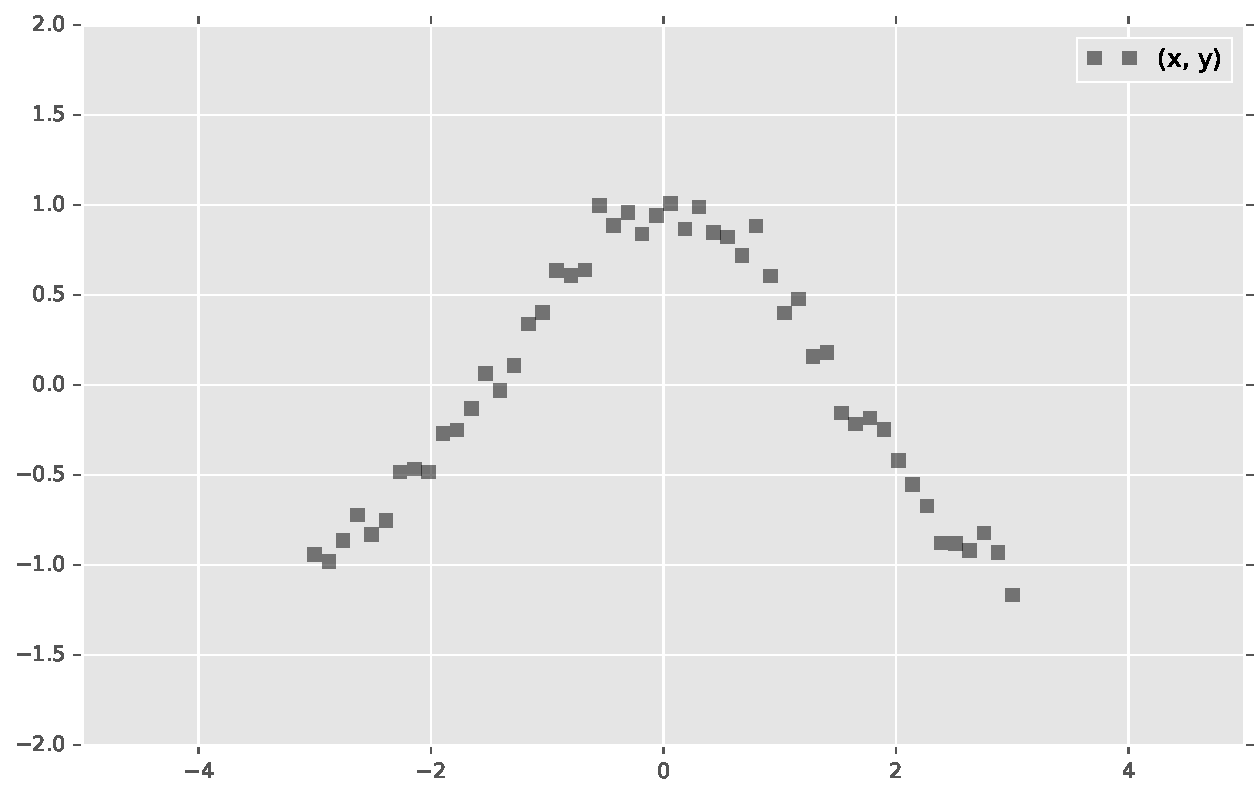
\includegraphics[width=3.5in]{images/getting-started-fig0.pdf}
\caption{Simulated data with a cosine relationship between $x$ and $y$.}
\end{figure}

Next, define a two-layer Bayesian neural network. Here, we
define the neural network manually with \texttt{tanh} nonlinearities.

\begin{lstlisting}[language=Python]
import tensorflow as tf
from edward.models import Normal

W_0 = Normal(mu=tf.zeros([1, 2]), sigma=tf.ones([1, 2]))
W_1 = Normal(mu=tf.zeros([2, 1]), sigma=tf.ones([2, 1]))
b_0 = Normal(mu=tf.zeros(2), sigma=tf.ones(2))
b_1 = Normal(mu=tf.zeros(1), sigma=tf.ones(1))

x = x_train
y = Normal(mu=tf.matmul(tf.tanh(tf.matmul(x, W_0) + b_0), W_1) + b_1,
           sigma=0.1)
\end{lstlisting}

Next, make inferences about the model from data. We will use variational
inference. Specify a normal approximation over the weights and biases.

\begin{lstlisting}[language=Python]
qW_0 = Normal(mu=tf.Variable(tf.zeros([1, 2])),
              sigma=tf.nn.softplus(tf.Variable(tf.zeros([1, 2]))))
qW_1 = Normal(mu=tf.Variable(tf.zeros([2, 1])),
              sigma=tf.nn.softplus(tf.Variable(tf.zeros([2, 1]))))
qb_0 = Normal(mu=tf.Variable(tf.zeros(2)),
              sigma=tf.nn.softplus(tf.Variable(tf.zeros(2))))
qb_1 = Normal(mu=tf.Variable(tf.zeros(1)),
              sigma=tf.nn.softplus(tf.Variable(tf.zeros(1))))
\end{lstlisting}

Defining \texttt{tf.Variable} allows the variational factors'
parameters to vary. They are all initialized at 0. The standard
deviation parameters are constrained to be greater than zero according
to a
softplus transformation\footnote{
The softplus function is defined as $\textrm{softplus}(x) =
\log(1+\exp(x))$.}.

Now, run variational inference with the
Kullback-Leibler divergence
in order to infer the model's latent variables given data.
We specify \texttt{1000} iterations.

\begin{lstlisting}[language=Python]
import edward as ed

inference = ed.KLqp({W_0: qW_0, b_0: qb_0,
                     W_1: qW_1, b_1: qb_1}, data={y: y_train})
inference.run(n_iter=1000)
\end{lstlisting}

Finally, criticize the model fit. Bayesian neural networks define a distribution
over neural networks, so we can perform a graphical check. Draw neural networks
from the inferred model and visualize how well it fits the data.

\begin{figure}[h]
\centering
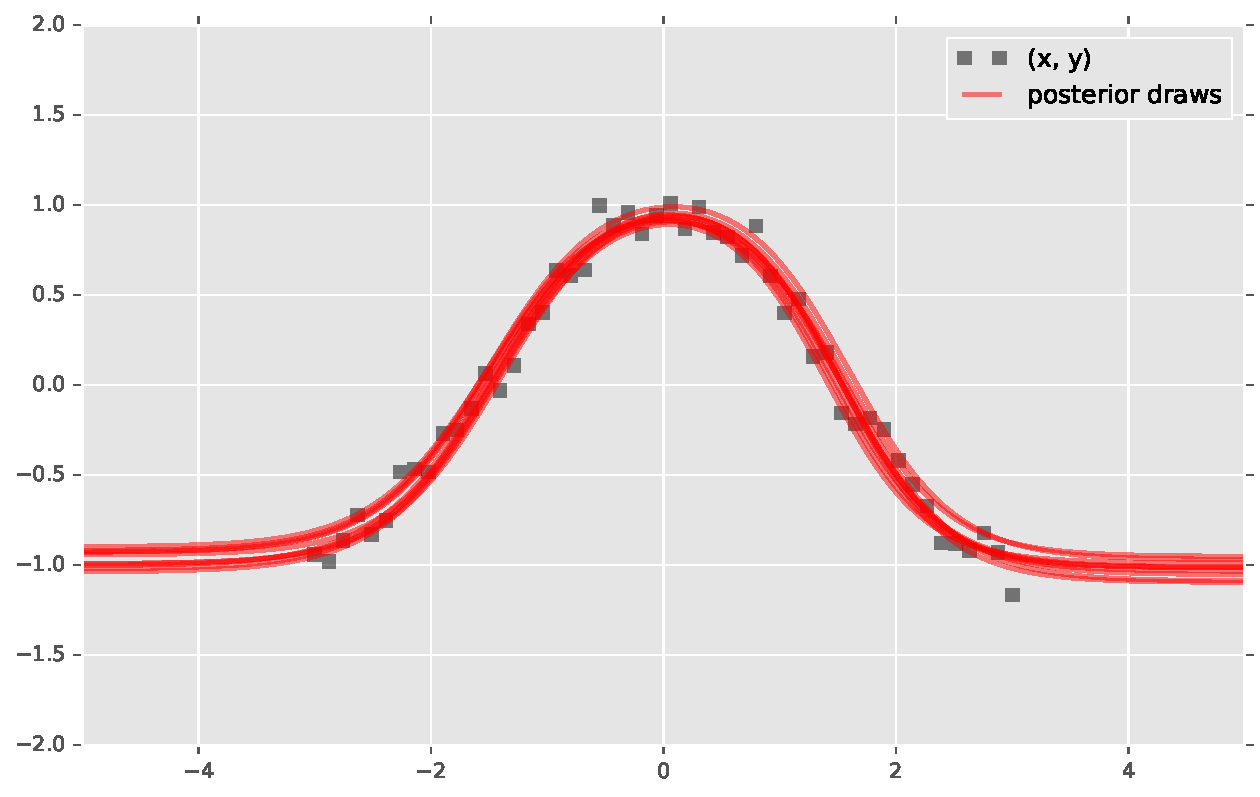
\includegraphics[width=3.5in]{images/getting-started-fig1.pdf}
\caption{Posterior draws from the inferred Bayesian neural network.}
\end{figure}

The model has captured the cosine relationship between $x$ and $y$
in the observed domain.

\clearpage
\section{Design}
\label{sec:design}

Edward's design reflects the building blocks for probabilistic
modeling. It defines interchangeable components, enabling rapid
experimentation and research with probabilistic models.

Edward is named after the innovative statistician
George Edward Pelham Box. Edward follows Box's philosophy of statistics and
machine learning \citep{box1976science}.

First gather data from some real-world phenomena. Then cycle through
Box's loop \citep{blei2014build}.

\begin{enumerate}
\item Build a probabilistic model of the phenomena.
\item Reason about the phenomena given model and data.
\item Criticize the model, revise and repeat.
\end{enumerate}

\begin{figure}[htb]
\centering
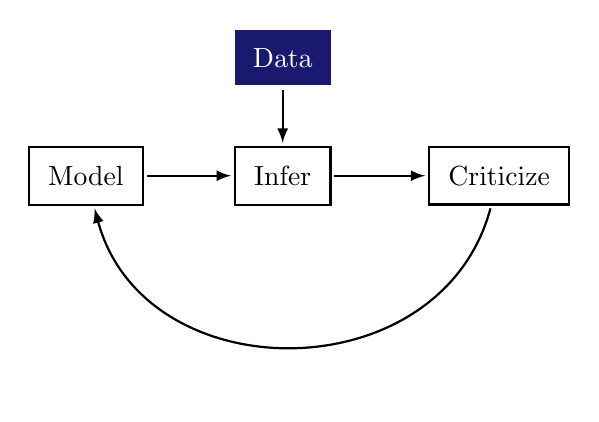
\begin{tikzpicture}
	\begin{pgfonlayer}{nodelayer}
		\node [style=box] (0) at (-2.5, 0) {Model};
		\node [style=box] (1) at (0, 0) {Infer};
		\node [style=box, fill=MidnightBlue, draw=white] (2) at (0, 1.5)
		{\color{white}Data};
		\node [style=box] (3) at (2.75, 0) {Criticize};
	\end{pgfonlayer}
	\begin{pgfonlayer}{edgelayer}
		\draw [style=arrow] (0) to (1);
		\draw [style=arrow] (2) to (1);
		\draw [style=arrow] (1) to (3);
		\draw [style=arrow, bend left=75, looseness=1.25] (3) to (0);
	\end{pgfonlayer}
\end{tikzpicture}

\caption{Box's loop.}
\end{figure}


Here's a toy example. A child flips a coin ten times, with the set of outcomes
being

\texttt{{[}0,\ 1,\ 0,\ 0,\ 0,\ 0,\ 0,\ 0,\ 0,\ 1{]}},

where \texttt{0}
denotes tails and \texttt{1} denotes heads. She is interested in the
probability that the coin lands heads. To analyze this, she first
builds a model: suppose she assumes the coin flips are independent and
land heads with the same probability. Second, she reasons about the
phenomenon: she infers the model's hidden structure given data.
Finally, she criticizes the model: she analyzes whether her model
captures the real-world phenomenon of coin flips. If it doesn't, then
she may revise the model and repeat.

We describe modules enabling this analysis.

\subsection{Data}

Data defines a set of observations. There are three ways
to read data in Edward.

\textbf{Preloaded data.}
A constant or variable in the TensorFlow graph holds all the data.
This setting is the fastest to work with and is recommended if the
data fits in memory.

Represent the data as NumPy arrays or TensorFlow tensors.

\begin{lstlisting}[language=Python]
x_data = np.array([0, 1, 0, 0, 0, 0, 0, 0, 0, 1])
x_data = tf.constant([0, 1, 0, 0, 0, 0, 0, 0, 0, 1])
\end{lstlisting}

During inference, we store them in TensorFlow variables internally to
prevent copying data more than once in memory.

\textbf{Feeding.}
Manual code provides the data when running each step of inference.
This setting provides the most fine control which is useful for
experimentation.

Represent the data as
TensorFlow placeholders,
which are nodes in the graph that are fed at runtime.

\begin{lstlisting}[language=Python]
x_data = tf.placeholder(tf.float32, [100, 25])  # placeholder of shape (100, 25)
\end{lstlisting}

During inference, the user must manually feed the placeholders. At each
step, call \texttt{inference.update()} while
passing in a \texttt{feed\_dict} dictionary
which binds placeholders to realized values as an argument.
If the values do not change over inference updates, one can also bind
the placeholder to values within the \texttt{data} argument when
first constructing inference.

\textbf{Reading from files.}
An input pipeline reads the data from files at the beginning of a
TensorFlow graph. This setting is recommended if the data does not
fit in memory.

\begin{lstlisting}[language=Python]
filename_queue = tf.train.string_input_producer(...)
reader = tf.SomeReader()
...
\end{lstlisting}

Represent the data as TensorFlow tensors, where the tensors are the
output of data readers. During inference, each update will be
automatically evaluated over new batch tensors represented through
the data readers.

\section{Compositional Representations for Probabilistic Models}
\label{sec:modeling_language}

We define random variables as a key compositional representation.
They are class objects with methods, for example, to compute the log density
and to sample. Further, each random variable $\mbx$ is associated to a
tensor $\mbx^*$ in the computational graph, which represents a single
sample $\mbx^*\sim p(\mbx)$.  This association embeds the random
variable into the computational graph.

This design is conceptually simple, making it easy to develop
probabilistic programs in a computational graph framework.
Importantly, all computation is represented on the graph.  This makes
it easy to parameterize random variables with complex deterministic
structure, such as with deep neural networks and a diverse set of math
operations.  The design also enables compositions of random variables
to capture complex stochastic structure.

With computational graphs, it is also natural to build mutable states
within the probabilistic program.  As a typical use of computational
graphs, such states can define model parameters; in TensorFlow, this
is given by a \texttt{tf.Variable}.  Another use case is for building
discriminative models $p(\mby\g\mbx)$, where
$\mbx$ are features that are input as training or test data.  The
program can be written independent of the data, using a mutable state
(\texttt{tf.placeholder}) for $\mbx$ in its graph.
During training and testing, we feed the placeholder the appropriate
values.
In \Cref{appendix:bnn}, we demonstrate this with a Bayesian neural
network for classification.
We give other examples below.


\subsection{Example: Variational Auto-encoder}

\begin{figure}[tb]
\begin{subfigure}{0.225\columnwidth}
  \centering
  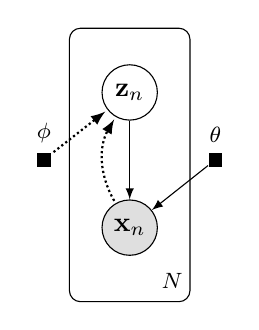
\begin{tikzpicture}

  % Nodes
  \node[latent] (z) {$\mbz_n$};
  \node[obs, below=of z] (x) {$\mbx_n$};

  \factor[empty, below=of z] {h} {} {} {};
  \factor[right=of h, xshift=0.5cm] {theta} {$\theta$} {} {};
  \factor[left=of h, xshift=-0.5cm] {phi} {$\phi$} {} {};

  % Edges
  \edge{z}{x};
  \draw[style=arrow, densely dotted, bend left] (x) to (z);
  \edge{theta}{x};
  \draw[style=arrow, densely dotted] (phi) to (z);

  % Plates
  \plate[inner sep=0.4cm, yshift=0.05cm,
    label={[xshift=-14pt,yshift=14pt]south east:$N$}] {plate1} {
    (z)(x)
  } {};

\end{tikzpicture}

  \label{sub:vae_math}
\end{subfigure}%
\begin{subfigure}{0.65\columnwidth}
  \centering
\begin{lstlisting}[language=python]
# Probabilistic model
z = Normal(mu=tf.zeros([N, d]), sigma=tf.ones([N, d]))
h = slim.fully_connected(z, 256)
x = Bernoulli(logits=slim.fully_connected(h, 28 * 28, activation_fn=None))

# Variational model
qx = tf.placeholder(tf.float32, [N, 28 * 28])
qh = slim.fully_connected(qx, 256)
qz = Normal(mu=slim.fully_connected(qh, d, activation_fn=None),
            sigma=slim.fully_connected(qh, d, activation_fn=tf.nn.softplus))
\end{lstlisting}
  \label{sub:vae_code}
\end{subfigure}
\caption{\Acrlong{VAE} for a data set of $28\times 28$ pixel images:
(left) graphical model, with dotted lines for the inference
model; (right) probabilistic program,
with 2-layer neural networks.
}
\label{fig:vae}
\end{figure}

\Cref{fig:vae}
implements
a \gls{VAE} \citep{kingma2014autoencoding,rezende2014stochastic} in Edward.
There are $N$ data points $\{x_n\}$ and $d$ latent
variables per data point $\{z_n\}$.
The program uses TensorFlow Slim \citep{guadarrama2016tensorflow}
to define the neural networks.
The probabilistic model is parameterized by a 2-layer neural network,
with 256 hidden units (and ReLU activation), and generates $28\times 28$
pixel images.  The variational model is parameterized by
a 2-layer inference network, with 256 hidden units and outputs
parameters of a normal posterior approximation.

The probabilistic program is concise.  Importantly, core elements of
the \gls{VAE}---such as its distributional assumptions and neural net
architectures---are all extensible.
Model compositionality enables it to be embedded into more complicated
models \citep{gregor2015draw,rezende2016one} and for other learning
tasks \citep{kingma2014semi}.
Inference compositionality (which we discuss later) enables it to be embedded into more
complicated algorithms, such as with expressive variational
approximations \citep{rezende2015variational,tran2016variational,kingma2016improving}
and alternative objectives \citep{ranganath2016operator,li2016variational,dieng2016chi}.


\subsection{Stochastic Control Flow and Model Parallelism}

\begin{figure}[!htb]
  \centering
  \begin{tikzpicture}[x=1.7cm,y=1.8cm,scale=0.9]
%\begin{tikzpicture}[scale=0.6]

  % Nodes
  \node[latent] (p) {$\mbp$};
  \factor[right=of p, xshift=0.3cm] {pstar} {$\mbp^*$} {} {};

  \factor[above=of pstar] {n} {} {} {};
  \factor[empty, right=of n, yshift=0.1cm] {nn} {\texttt{tf.while_loop(...)}} {} {};
  \factor[left=of n, xshift=-0.5cm] {astar} {$\mba^*$} {} {};
  \node[latent, left=of astar, xshift=0.5cm] (a) {$\mba$};
  \node[latent, right=of pstar, xshift=-0.5cm] (x) {$\mbx$};
  \factor[right=of x, xshift=0.3cm] {xstar} {$\mbx^*$} {} {};

  % Edges
  \edge{p}{pstar};
  \edge{pstar}{x};
  \edge{n}{x};
  \edge{x}{xstar};
  \edge{a}{astar};
  \edge{astar}{n};

\end{tikzpicture}

\caption{Computational graph for a probabilistic program with stochastic control flow.
}
\label{fig:dynamic}
\end{figure}

Random variables can also be integrated with control flow,
enabling probabilistic programs with stochastic control flow.
%
Stochastic control flow defines dynamic conditional dependencies,
known in the literature as contingent or existential dependencies
\citep{mansinghka2014venture,wu2016swift}.
See \Cref{fig:dynamic}, where $\mbx$ may or may not depend on $\mba$
for a given execution.

We use stochastic control flow to implement a Dirichlet process mixture model
in \Cref{appendix:dirichlet_process}.
Stochastic control flow produces difficulties for algorithms that leverage the
graph structure; the relationship of conditional dependencies
changes across execution traces.
Importantly, the computational graph provides
an elegant way of teasing out static conditional dependence structure
($\mbp$) from dynamic dependence structure ($\mba)$.  We can perform
model parallelism over the static structure with \glspl{GPU} and batch
training, and use generic computations to handle the dynamic
structure.

\subsection*{Composing Random Variables}

Core to Edward's design is compositionality. Compositionality enables
fine control of modeling, where models are represented as a collection
of random variables.

We outline how to write popular classes of models using Edward:
directed graphical models, neural networks, Bayesian nonparametrics,
and probabilistic programs.

\subsubsection{Directed Graphical Models}

Graphical models are a rich formalism for specifying probability
distributions \citep{koller2009probabilistic}.
In Edward, directed edges in a graphical model are implicitly defined
when random variables are composed with one another. We illustrate
with a Beta-Bernoulli model,
\begin{equation*}
p(\mathbf{x}, \theta) =
\text{Beta}(\theta\mid 1, 1)
\prod_{n=1}^{50} \text{Bernoulli}(x_n\mid \theta),
\end{equation*}
where $\theta$ is a latent probability shared across the 50 data
points $\mathbf{x}\in\{0,1\}^{50}$.

\begin{lstlisting}[language=python]
from edward.models import Bernoulli, Beta

theta = Beta(a=1.0, b=1.0)
x = Bernoulli(p=tf.ones(50) * theta)
\end{lstlisting}

\begin{figure}[!htb]
\centering
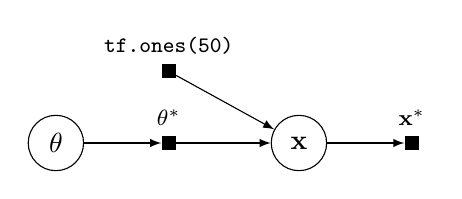
\begin{tikzpicture}[x=1.7cm,y=1.8cm,scale=0.9]
%\begin{tikzpicture}[scale=0.6]

  % Nodes
  \node[latent] (theta) {$\theta$};
  \factor[right=of theta, xshift=0.3cm] {thetastar} {$\theta^*$} {} {};

  \factor[above=of thetastar] {n} {\texttt{tf.ones(50)}} {} {};
  \node[latent, right=of thetastar, xshift=-0.5cm] (x) {$\mbx$};
  \factor[right=of x, xshift=0.3cm] {xstar} {$\mbx^*$} {} {};

  % Edges
  \edge{theta}{thetastar};
  \edge{thetastar}{x};
  \edge{n}{x};
  \edge{x}{xstar};

\end{tikzpicture}

\caption{Computational graph for a Beta-Bernoulli program.}
\end{figure}

The random variable \texttt{x} ($\mathbf{x}$) is 50-dimensional,
parameterized by the random tensor $\theta^*$. Fetching the object
\texttt{x.value()} ($\mathbf{x}^*$) from session runs the graph: it simulates from
the generative process and outputs a binary vector of $50$ elements.

With computational graphs, it is also natural to build mutable states
within the probabilistic program. As a typical use of computational
graphs, such states can define model parameters, that is, parameters
that we will always compute point estimates for and not be uncertain
about. In TensorFlow, this is given by a \texttt{tf.Variable}.

\begin{lstlisting}[language=python]
from edward.models import Bernoulli

theta = tf.Variable(0.0)
x = Bernoulli(p=tf.ones(50) * tf.sigmoid(theta))
\end{lstlisting}

Another use case of mutable states is for building discriminative
models $p(\mathbf{y}\mid\mathbf{x})$, where $\mathbf{x}$ are features
that are input as training or test data. The program can be written
independent of the data, using a mutable state
(\texttt{tf.placeholder}) for $\mathbf{x}$ in its graph. During
training and testing, we feed the placeholder the appropriate values.

\subsubsection{Neural Networks}

As Edward uses TensorFlow, it is easy to construct neural networks for
probabilistic modeling \citep{rumelhart1988parallel}.
For example, one can specify stochastic neural networks
\citep{neal1990learning}.

High-level libraries such as
{Keras}\footnote{\url{http://keras.io}} and
{TensorFlow Slim}\footnote{\url{https://github.com/tensorflow/tensorflow/tree/master/tensorflow/contrib/slim}}
can be used to easily construct deep neural networks.
We illustrate this with a deep generative model over binary data
$\{\mathbf{x}_n\}\in\{0,1\}^{N\times 28*28}$.

\begin{figure}[!htb]
\centering
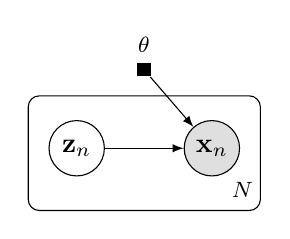
\begin{tikzpicture}

  % Nodes
  \node[latent] (z) {$\mbz_n$};
  \node[obs, right=of z] (x) {$\mbx_n$};

  \factor[empty, right=of z] {h} {} {} {};
  \factor[right=of z, yshift=1.0cm] {theta} {$\theta$} {} {};
  % \factor[left=of h, xshift=-0.5cm] {phi} {$\phi$} {} {};

  % Edges
  \edge{z}{x};
  % \draw[style=arrow, densely dotted, bend left] (x) to (z);
  \edge{theta}{x};
  % \draw[style=arrow, densely dotted] (phi) to (z);

  % Plates
  \plate[inner sep=0.25cm, yshift=0.05cm,
    label={[xshift=-14pt,yshift=14pt]south east:$N$}] {plate1} {
    (z)(x)
  } {};

\end{tikzpicture}

\caption{Graphical representation of a deep generative model.}
\end{figure}

The model specifies a generative process where for each
$n=1,\ldots,N$,
%
\begin{align*}
\mathbf{z}_n &\sim \text{Normal}(\mathbf{z}_n \mid \mathbf{0}, \mathbf{I}), \\
\mathbf{x}_n\mid \mathbf{z}_n &\sim \text{Bernoulli}(\mathbf{x}_n\mid
p=\mathrm{NN}(\mathbf{z}_n; \mathbf{\theta})).
\end{align*}
%
The latent space is $\mathbf{z}_n\in\mathbb{R}^d$ and the
likelihood is parameterized by a neural network $\mathrm{NN}$ with
parameters $\theta$. We will use a two-layer neural network with a
fully connected hidden layer of 256 units (with ReLU activation) and
whose output is $28*28$-dimensional. The output will be unconstrained,
parameterizing the logits of the Bernoulli likelihood.

With TensorFlow Slim, we write this model as follows:

\begin{lstlisting}[language=python]
from edward.models import Bernoulli, Normal
from tensorflow.contrib import slim

z = Normal(mu=tf.zeros([N, d]), sigma=tf.ones([N, d]))
h = slim.fully_connected(z, 256)
x = Bernoulli(logits=slim.fully_connected(h, 28 * 28, activation_fn=None))
\end{lstlisting}

With Keras, we write this model as follows:

\begin{lstlisting}[language=python]
from edward.models import Bernoulli, Normal
from keras.layers import Dense

z = Normal(mu=tf.zeros([N, d]), sigma=tf.ones([N, d]))
h = Dense(256, activation='relu')(z.value())
x = Bernoulli(logits=Dense(28 * 28)(h))
\end{lstlisting}

Keras and TensorFlow Slim automatically manage TensorFlow variables, which
serve as parameters of the high-level neural network layers. This
saves the trouble of having to manage them manually. However, note
that neural network parameters defined this way always serve as model
parameters. That is, the parameters are not exposed to the user so we
cannot be Bayesian about them with prior distributions.

\subsubsection{Bayesian Nonparametrics}

Bayesian nonparametrics enable rich probability models by working over
an infinite-dimensional parameter space \citep{hjort2010bayesian}.
Edward supports the two typical approaches to handling these models:
collapsing the infinite-dimensional space and lazily defining the
infinite-dimensional space.

For the collapsed approach, see the
Gaussian process classification
tutorial as an example. We specify distributions over the function
evaluations of the Gaussian process, and the Gaussian process is
implicitly marginalized out. This approach is also useful for Poisson
process models.

To work directly on the infinite-dimensional space, one can leverage
random variables with
control flow operations
in TensorFlow. At runtime, the control flow will lazily define any
parameters in the space necessary in order to generate samples. As an
example, we use a while loop to define a
Dirichlet process according to its stick breaking representation.

\subsubsection{Probabilistic Programs}

Probabilistic programs greatly expand the scope of probabilistic
models \citep{goodman2012church}.
Formally, Edward is a Turing-complete probabilistic programming
language. This means that Edward can represent any computable
probability distribution.

\begin{figure}[!htb]
\centering
\begin{tikzpicture}[x=1.7cm,y=1.8cm,scale=0.9]
%\begin{tikzpicture}[scale=0.6]

  % Nodes
  \node[latent] (p) {$\mbp$};
  \factor[right=of p, xshift=0.3cm] {pstar} {$\mbp^*$} {} {};

  \factor[above=of pstar] {n} {} {} {};
  \factor[empty, right=of n, yshift=0.1cm] {nn} {\texttt{tf.while_loop(...)}} {} {};
  \factor[left=of n, xshift=-0.5cm] {astar} {$\mba^*$} {} {};
  \node[latent, left=of astar, xshift=0.5cm] (a) {$\mba$};
  \node[latent, right=of pstar, xshift=-0.5cm] (x) {$\mbx$};
  \factor[right=of x, xshift=0.3cm] {xstar} {$\mbx^*$} {} {};

  % Edges
  \edge{p}{pstar};
  \edge{pstar}{x};
  \edge{n}{x};
  \edge{x}{xstar};
  \edge{a}{astar};
  \edge{astar}{n};

\end{tikzpicture}

\caption{Computational graph for a probabilistic program with stochastic control flow.}
\end{figure}

Random variables can be composed with control flow operations,
enabling probabilistic programs with stochastic control flow.
%
Stochastic control flow defines dynamic conditional dependencies,
known in the literature as contingent or existential dependencies
\citep{mansinghka2014venture,wu2016swift}.
See above, where $\mathbf{x}$ may or may not depend on $\mathbf{a}$
for a given execution.

Stochastic control flow produces difficulties for algorithms that
leverage the graph structure; the relationship of conditional
dependencies changes across execution traces.
Importantly, the computational graph provides an elegant way of
teasing out static conditional dependence structure ($\mathbf{p}$)
from dynamic dependence structure ($\mathbf{a})$. We can perform
model parallelism over the static structure with GPUs and batch
training, and use generic computations to handle the dynamic
structure.

\subsection*{Developing Custom Random Variables}

Oftentimes we'd like to implement our own random variables.
To do so, write a class that inherits
the \texttt{RandomVariable} class in \texttt{edward.models} and
the \texttt{Distribution} class in \texttt{tf.contrib.distributions} (in that
order). A template is provided below.

\begin{lstlisting}[language=Python]
from edward.models import RandomVariable
from tensorflow.contrib.distributions import Distribution

class CustomRandomVariable(RandomVariable, Distribution):
  def __init__(self, *args, **kwargs):
    super(CustomRandomVariable, self).__init__(*args, **kwargs)

  def _log_prob(self, value):
    raise NotImplementedError("log_prob is not implemented")

  def _sample_n(self, n, seed=None):
    raise NotImplementedError("sample_n is not implemented")
\end{lstlisting}

One method that all Edward random variables call during instantiation is
\texttt{_sample_n()}.
It takes an integer \texttt{n} as input and outputs a tensor of shape
\texttt{(n,) + batch_shape + event_shape}.
To implement it, you can for example wrap a NumPy/SciPy function
inside the TensorFlow operation \texttt{tf.py_func()}.

For other methods and attributes one can implement, see the API documentation in
TensorFlow's
\texttt{Distribution} class.

\subsubsection{Advanced settings}

Sometimes the random variable you'd like to work with already exists
in Edward, but it is missing a particular feature. One hack is to
implement and overwrite the missing method. For example, to implement
your own sampling for \texttt{Poisson}:

\begin{lstlisting}[language=Python]
import edward as ed
from edward.models import Poisson
from scipy.stats import poisson

def _sample_n(self, n=1, seed=None):
  # define Python function which returns samples as a Numpy array
  def np_sample(lam, n):
    return poisson.rvs(mu=lam, size=n, random_state=seed).astype(np.float32)

  # wrap python function as tensorflow op
  val = tf.py_func(np_sample, [self.lam, n], [tf.float32])[0]
  # set shape from unknown shape
  batch_event_shape = self.get_batch_shape().concatenate(self.get_event_shape())
  shape = tf.concat([tf.expand_dims(n, 0),
                     tf.constant(batch_event_shape.as_list(), dtype=tf.int32)],
                     0)
  val = tf.reshape(val, shape)
  return val

Poisson._sample_n = _sample_n

sess = ed.get_session()
x = Poisson(lam=1.0)
sess.run(x.value())
## 1.0
sess.run(x.value())
## 4.0
\end{lstlisting}

(Note the function \texttt{np_sample} should broadcast correctly if
you'd like to work with non-scalar parameters; it is not correct in
this toy implementation.)

Sometimes the random variable you'd like to work with does not even
admit (easy) sampling, and you're only using it as a likelihood ``node'' rather
than as some prior to parameters of another random variable.
You can avoid having to implement \texttt{_sample_n} altogether:
after creating \texttt{CustomRandomVariable}, instantiate it with the
\texttt{value} argument:

\begin{lstlisting}[language=Python]
x = CustomRandomVariable(custom_params=params, value=tf.zeros_like(params))
\end{lstlisting}

This fixes the associated value of the random variable to a bunch of
zeros and avoids the \texttt{_sample_n} error that appears otherwise.
Make sure that the value matches the desired shape of the random
variable.

\section{Compositional Representations for Inference}
\label{sec:inference}

We described random variables as a representation for building
rich probabilistic programs over computational graphs.  We now
describe a compositional representation for inference.
We desire two criteria: (a) support for many classes of
inference, where the form of the inferred posterior depends on the
algorithm; and (b) invariance of inference under the computational
graph, that is, the posterior can be further composed as part of
another model.

To explain our approach, we will use a simple hierarchical model as a
running example. \Cref{fig:hierarchical_model_example} displays a
joint distribution $p(\mbx, \mbz, \beta)$ of data $\mbx$, local
variables $\mbz$, and global variables $\beta$. The ideas here extend
to more expressive programs.

\begin{figure}[!h]
\begin{subfigure}{0.35\columnwidth}
  \centering
  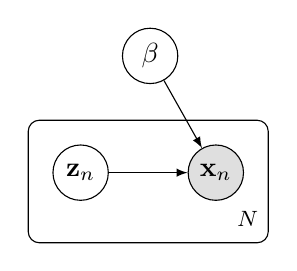
\begin{tikzpicture}

  % Nodes
  \node[latent]               (beta)      {$\beta$} ;
  \node[left=0.4cm of beta]               (betaph)      {} ;
  \node[latent, below=1.0cm of betaph] (z)    {$\mbz_n$} ;
  \node[obs, right=1.0cm of z]      (x)        {$\mbx_n$} ;

  % Edges
  % \edge{beta}{z};
  \edge{beta}{x};
  \edge{z}{x};

  % Plates
  \plate[inner sep=0.3cm,
    label={[xshift=-15pt,yshift=15pt]south east:$N$}] {plate1} {
    (x)(z)
  } {};

\end{tikzpicture}

\end{subfigure}%
\begin{subfigure}{0.6\columnwidth}
  \centering
\begin{lstlisting}[language=python]
N = 10000  # number of data points
D = 2  # data dimension
K = 5  # number of clusters

beta = Normal(mu=tf.zeros([K, D]), sigma=tf.ones([K, D]))
z = Categorical(logits=tf.zeros([N, K]))
x = Normal(mu=tf.gather(beta, z), sigma=tf.ones([N, D]))
\end{lstlisting}
\end{subfigure}
\caption{Hierarchical model: \textbf{(left)} graphical model; \textbf{(right)}
  probabilistic program. It is a mixture of Gaussians over
  $D$-dimensional data $\{x_n\}\in\mathbb{R}^{N\times D}$. There are
  $K$ latent cluster means $\beta\in\mathbb{R}^{K\times D}$.}
\label{fig:hierarchical_model_example}
\end{figure}

\subsection{Inference as Stochastic Graph Optimization}
\label{sub:inference}

The goal of inference is to
calculate the posterior distribution
$p(\mathbf{z}, \beta\mid \mathbf{x}_{\text{train}}; \mbtheta)$
given data $\mbx_{\text{train}}$,
where
$\mbtheta$ are any model parameters that we will compute point estimates
for.\footnote{%
For example, we could replace \texttt{x}'s \texttt{sigma}
argument with \texttt{tf.exp(tf.Variable(0.0))*tf.ones([N, D])}. This
defines a model parameter initialized at 0 and positive-constrained.}
We formalize this as the following optimization problem:
\begin{align}
  \label{eq:inference-optimization}
\min_{\mblambda,\mbtheta}
\mathcal{L}(
p(\mathbf{z}, \beta\mid \mathbf{x}_{\text{train}}; \mbtheta),~
q(\mathbf{z}, \beta; \mblambda)
),
\end{align}
where $q(\mathbf{z}, \beta; \mblambda)$ is an approximation to the
posterior $p(\mathbf{z}, \beta\g \mbx_{\text{train}};\mbtheta)$, and
$\mathcal{L}$ is a loss function with respect to $p$ and $q$.

The choice of approximation $q$, loss $\mathcal{L}$, and rules to update
parameters $\{\mbtheta,\mblambda\}$ are specified by an inference algorithm.
(Note $q$ can be nonparametric, such as a point or a collection of
samples.)

In Edward, we write this problem as follows:

\begin{lstlisting}[language=python]
inference = ed.Inference({beta: qbeta, z: qz}, data={x: x_train})
\end{lstlisting}

\texttt{Inference} is an abstract class which takes two inputs.  The
first is a collection of latent random variables \texttt{beta} and
\texttt{z}, associated to their ``posterior variables'' \texttt{qbeta} and
\texttt{qz} respectively. The second is a collection of observed random variables
\texttt{x}, which is associated to their realizations \texttt{x_train}.

The idea is that \texttt{Inference} defines and
solves the optimization in \Cref{eq:inference-optimization}. It
adjusts parameters of the distribution of \texttt{qbeta}
and \texttt{qz} (and any model parameters) to be close to the
posterior.

Class methods are available to finely control the inference. Calling
\texttt{inference.initialize()} builds a computational graph to update
$\{\mbtheta,\mblambda\}$. Calling \texttt{inference.update()} runs
this computation once to update $\{\mbtheta,\mblambda\}$; we call the
method in a loop until convergence. Importantly, no efficiency is lost
in Edward's language: the computational graph is the same as if it
were handwritten for a
specific model. This means the runtime is the same; also see our
experiments in \Cref{sub:gpu}.

A key concept in Edward is that there is no distinct ``model''
or ``inference'' block. A model is simply a collection of random
variables, and inference is a way of modifying parameters in that
collection subject to another. This reductionism offers
significant flexibility. For example, we can
infer only parts of a model (e.g.,
layer-wise training \citep{hinton2006fast}),
infer parts used in multiple models
(e.g., multi-task learning), or
plug in a posterior into a new model
(e.g., Bayesian updating).

\subsection{Classes of Inference}

The design of \texttt{Inference} is very general.  We describe
subclasses to represent many algorithms below: variational inference,
Monte Carlo, and \acrlongpl{GAN}.

Variational inference posits a family of approximating distributions
and finds the closest member in the family to the posterior
\citep{jordan1999introduction}.  In Edward, we build the variational
family in the graph; see \Cref{fig:inference} (left). For our running
example, the
family has mutable variables as parameters
$\mblambda=\{\pi,\mu,\sigma\}$, where
$q(\beta;\mu,\sigma) = \operatorname{Normal}(\beta; \mu,\sigma)$ and
$q(\mbz;\pi) = \operatorname{Categorical}(\mbz;\pi)$.

\begin{figure}[!h]
\begin{subfigure}{0.5\columnwidth}
  \centering
\begin{lstlisting}[language=Python]
qbeta = Normal(
  mu=tf.Variable(tf.zeros([K, D])),
  sigma=tf.exp(tf.Variable(tf.zeros([K, D]))))
qz = Categorical(
  logits=tf.Variable(tf.zeros([N, K])))

inference = ed.VariationalInference(
  {beta: qbeta, z: qz}, data={x: x_train})
\end{lstlisting}
\end{subfigure}%
\begin{subfigure}{0.5\columnwidth}
  \centering
\begin{lstlisting}[language=Python]
T = 10000  # number of samples
qbeta = Empirical(
  params=tf.Variable(tf.zeros([T, K, D])))
qz = Empirical(
  params=tf.Variable(tf.zeros([T, N])))

inference = ed.MonteCarlo(
  {beta: qbeta, z: qz}, data={x: x_train})
\end{lstlisting}
\end{subfigure}
\caption{\textbf{(left)} Variational inference. \textbf{(right)} Monte Carlo.}
\label{fig:inference}
\end{figure}

Specific variational algorithms inherit from the
\texttt{VariationalInference} class.  Each defines its own methods,
such as a loss function and gradient.
For example, we represent
\gls{MAP}
estimation with an approximating family (\texttt{qbeta} and
\texttt{qz}) of \texttt{PointMass} random variables, i.e., with all
probability mass concentrated at a point.
\texttt{MAP} inherits from \texttt{VariationalInference} and defines
the negative log joint density as the loss function; it uses existing optimizers inside
TensorFlow.
In \Cref{sub:recent}, we experiment with multiple gradient estimators
for black box variational inference \citep{ranganath:2014}. Each
estimator implements the same loss (an objective proportional to
the divergence $\operatorname{KL}(q\gg p)$) and a different update rule
(stochastic gradient).

Monte Carlo approximates the posterior using samples
\citep{robert1999monte}. Monte Carlo is an inference where the
approximating family is an empirical distribution,
$q(\beta; \{\beta^{(t)}\}) = \frac{1}{T}\sum_{t=1}^T \delta(\beta,
\beta^{(t)})$ and
$q(\mbz; \{\mbz^{(t)}\}) = \frac{1}{T}\sum_{t=1}^T \delta(\mbz,
\mbz^{(t)})$. The parameters are
$\mblambda=\{\beta^{(t)},\mbz^{(t)}\}$.  See \Cref{fig:inference}
(right).
Monte Carlo algorithms proceed by updating one sample
$\beta^{(t)},\mbz^{(t)}$ at a time in the empirical approximation.
Specific \glsunset{MC}\gls{MC} samplers determine the update rules:
they can use gradients such as in Hamiltonian Monte Carlo
\citep{neal2011mcmc} and graph
structure such as in sequential Monte Carlo \citep{doucet2001introduction}.



\begin{figure}[tb]
\begin{subfigure}{0.4\columnwidth}
  \centering
  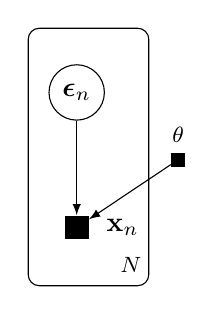
\begin{tikzpicture}

  % Nodes
  \node[latent] (eps0) {$\mbepsilon_n$};
  \factor[minimum size=0.3cm, below=1.2cm of eps0] {x} {} {} {};

  \factor[empty, below=of eps0] {h} {} {} {};
  \factor[right=of h, xshift=0.7cm] {theta} {$\theta$} {} {};

  \node[right=of x, xshift=-0.9cm] (xlabel) {$\mbx_n$};

  % Edges
  \edge{eps0}{x};
  \edge{theta}{x};

  % Plates
  \plate[inner sep=0.4cm, yshift=0.05cm,xshift=0.15cm,
    label={[xshift=-14pt,yshift=14pt]south east:$N$}] {plate1} {
    (eps0)(x)
  } {};

\end{tikzpicture}

\end{subfigure}%
\begin{subfigure}{0.6\columnwidth}
  \centering
\begin{lstlisting}[language=python]
def generative_network(eps):
  h = Dense(256, activation='relu')(eps)
  return Dense(28 * 28, activation=None)(h)

def discriminative_network(x):
  h = Dense(28 * 28, activation='relu')(x)
  return Dense(h, activation=None)(1)

# Probabilistic model
eps = Normal(mu=tf.zeros([N, d]), sigma=tf.ones([N, d]))
x = generative_network(eps)

inference = ed.GANInference(data={x: x_train},
    discriminator=discriminative_network)
\end{lstlisting}
\end{subfigure}
\caption{\Acrlongpl{GAN}:
\textbf{(left)} graphical model; \textbf{(right)} probabilistic program.
The model (generator) uses a parameterized function (discriminator)
for training.
}
\label{fig:gan}
\end{figure}

Edward also supports non-Bayesian methods such as \glspl{GAN}
\citep{goodfellow2014generative}.
See \Cref{fig:gan}.
The model posits
random noise \texttt{eps} over $N$ data points, each with $d$
dimensions; this random noise feeds into a
\texttt{generative_network} function, a neural network that outputs
real-valued data \texttt{x}.
In addition, there is a \texttt{discriminative_network}
which takes data as input and outputs the probability that
the data is real (in logit parameterization). We build
\texttt{GANInference}; running it optimizes parameters inside the two
neural network functions. This approach extends to many advances in
\glspl{GAN} (e.g., \citet{denton2015deep,li2015generative}).

Finally, one can design algorithms that would otherwise require tedious
algebraic manipulation. With symbolic algebra on nodes of the
computational graph, we can uncover conjugacy relationships between
random variables. Users can then integrate out variables to
automatically derive classical Gibbs \citep{gelfand1990sampling},
mean-field updates \citep{bishop2006pattern}, and exact inference.
These algorithms are being currently developed in Edward.

\subsection{Composing Inferences}

Core to Edward's design is that inference can be written as a collection
of separate inference programs. Below we demonstrate variational EM,
with an (approximate) E-step over local variables and an M-step over
global variables. We instantiate two algorithms, each of which
conditions on inferences from the other, and
we alternate with one update of each \citep{neal1993new},
\begin{lstlisting}[language=Python]
qbeta = PointMass(params=tf.Variable(tf.zeros([K, D])))
qz = Categorical(logits=tf.Variable(tf.zeros([N, K])))

inference_e = ed.VariationalInference({z: qz}, data={x: x_train, beta: qbeta})
inference_m = ed.MAP({beta: qbeta}, data={x: x_train, z: qz})
...
for _ in range(10000):
  inference_e.update()
  inference_m.update()
\end{lstlisting}
This extends to many other cases such as
exact EM for exponential families,
contrastive divergence \citep{hinton2002training},
pseudo-marginal methods \citep{andrieu2009pseudo},
and Gibbs sampling within variational inference
\citep{wang2012truncation,Hoffman:2015}.
We can also write message passing algorithms, which solve a collection
of local inference problems \citep{koller2009probabilistic}.  For
example, classical message passing uses exact local inference and
expectation propagation locally minimizes the Kullback-Leibler
divergence, $\text{KL}(p\gg q)$
\citep{minka2001expectation}.

\subsection{Data Subsampling}
\label{sub:batch_training}

Stochastic optimization \citep{bottou2010large} scales inference to
massive data and is key to
algorithms such as stochastic gradient Langevin dynamics
\citep{welling2011bayesian} and stochastic variational inference
\citep{hoffman2013stochastic}.  The idea is to cheaply estimate the
model's log joint density in an unbiased way.  At each step, one
subsamples a data set $\{x_m\}$ of size $M$ and then scales densities
with respect to local variables,
\begin{align*}
  \log p(\mbx, \mbz, \beta)
  & = \log p(\beta) +
  \sum_{n=1}^N\Big[\log p(x_n \g z_n, \beta) + \log p(z_n \g \beta)\Big]
  \\
  & \approx \log p(\beta) +
  \frac{N}{M}\sum_{m=1}^M\Big[\log p(x_m \g z_m, \beta) + \log p(z_m \g \beta)\Big].
\end{align*}
To support stochastic optimization, we represent only a subgraph of
the full model. This prevents reifying the full model, which can lead
to unreasonable memory consumption \citep{tristan2014augur}.  During
initialization, we pass in a dictionary to properly scale the
arguments. See \Cref{fig:hierachical_model_batch}.

\begin{figure}[!htb]
\begin{subfigure}{0.3\columnwidth}
  \centering
  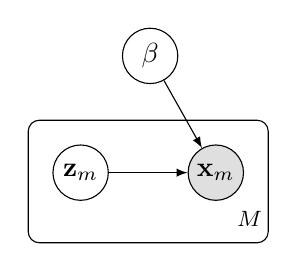
\begin{tikzpicture}

  % Nodes
  \node[latent]               (beta)      {$\beta$} ;
  \node[left=0.4cm of beta]               (betaph)      {} ;
  \node[latent, below=1.0cm of betaph] (z)    {$\mbz_m$} ;
  \node[obs, right=1.0cm of z]      (x)        {$\mbx_m$} ;

  % Edges
  % \edge{beta}{z};
  \edge{beta}{x};
  \edge{z}{x};

  % Plates
  \plate[inner sep=0.3cm,
    label={[xshift=-15pt,yshift=15pt]south east:$M$}] {plate1} {
    (x)(z)
  } {};

\end{tikzpicture}

  \label{sub:hierachical_model_math}
\end{subfigure}%
\begin{subfigure}{0.6\columnwidth}
  \centering
\begin{lstlisting}[language=python]
beta = Normal(mu=tf.zeros([K, D]), sigma=tf.ones([K, D]))
z = Categorical(logits=tf.zeros([M, K]))
x = Normal(mu=tf.gather(beta, z), sigma=tf.ones([M, D]))

qbeta = Normal(mu=tf.Variable(tf.zeros([K, D])),
               sigma=tf.nn.softplus(tf.Variable(tf.zeros([K, D]))))
qz = Categorical(logits=tf.Variable(tf.zeros([M, D])))

inference = ed.VariationalInference({beta: qbeta, z: qz}, data={x: x_batch})
inference.initialize(scale={x: float(N)/M, z: float(N)/M})
\end{lstlisting}
  \label{sub:hierarchical_model_code}
\end{subfigure}
\caption{Data subsampling with a hierarchical model. We define a
subgraph of the full model, forming a plate of size $M$
rather than $N$. We then scale all local random variables by $N/M$.}
\label{fig:hierachical_model_batch}
\end{figure}

Conceptually, the scale argument represents scaling for each random
variable's plate, as if we had seen that random variable $N / M$ as
many times.  As an example, \Cref{appendix:svi} shows how to implement
stochastic variational inference in Edward.
The approach extends naturally to streaming data
\citep{doucet2000on,broderick2013streaming,mcinerney2015population},
dynamic batch sizes, and data structures in which working on a
subgraph does not immediately apply
\citep{binder1997space,johnson2014stochastic,foti2014stochastic}.


\subsection*{Classes of Inference}

Inference is broadly classified under three classes: variational
inference, Monte Carlo, and exact inference.
We highlight how to use inference algorithms from each class.

As an example, we assume a mixture model with latent mixture
assignments \texttt{z}, latent cluster means \texttt{beta}, and
observations \texttt{x}:
\begin{equation*}
p(\mathbf{x}, \mathbf{z}, \beta)
=
\text{Normal}(\mathbf{x} \mid \beta_{\mathbf{z}}, \mathbf{I})
~
\text{Categorical}(\mathbf{z}\mid \pi)
~
\text{Normal}(\beta\mid \mathbf{0}, \mathbf{I}).
\end{equation*}

\subsubsection{Variational Inference}

In variational inference, the idea is to posit a family of approximating
distributions and to find the closest member in the family to the
posterior \citep{jordan1999introduction}.
We write an approximating family,
\begin{align*}
q(\beta;\mu,\sigma) &= \text{Normal}(\beta; \mu,\sigma), \\[1.5ex]
q(\mathbf{z};\pi) &= \text{Categorical}(\mathbf{z};\pi),
\end{align*}
using TensorFlow variables to represent its parameters
$\lambda=\{\pi,\mu,\sigma\}$.
\begin{lstlisting}[language=Python]
from edward.models import Categorical, Normal

qbeta = Normal(mu=tf.Variable(tf.zeros([K, D])),
               sigma=tf.exp(tf.Variable(tf.zeros[K, D])))
qz = Categorical(logits=tf.Variable(tf.zeros[N, K]))

inference = ed.VariationalInference({beta: qbeta, z: qz}, data={x: x_train})
\end{lstlisting}
Given an objective function, variational inference optimizes the
family with respect to \texttt{tf.Variable}s.

Specific variational inference algorithms inherit from
the \texttt{VariationalInference} class to define their own methods, such as a
loss function and gradient.
For example, we represent
MAP
estimation with an approximating family (\texttt{qbeta} and
\texttt{qz}) of \texttt{PointMass} random variables, i.e., with all
probability mass concentrated at a point.
\begin{lstlisting}[language=Python]
from edward.models import PointMass

qbeta = PointMass(params=tf.Variable(tf.zeros([K, D])))
qz = PointMass(params=tf.Variable(tf.zeros(N)))

inference = ed.MAP({beta: qbeta, z: qz}, data={x: x_train})
\end{lstlisting}
\texttt{MAP} inherits from \texttt{VariationalInference} and defines a
loss function and update rules; it uses existing optimizers inside
TensorFlow.

\subsubsection{Monte Carlo}

Monte Carlo approximates the posterior using samples
\citep{robert1999monte}. Monte Carlo is an inference where the
approximating family is an empirical distribution,
\begin{align*}
q(\beta; \{\beta^{(t)}\})
&= \frac{1}{T}\sum_{t=1}^T \delta(\beta, \beta^{(t)}), \\[1.5ex]
q(\mathbf{z}; \{\mathbf{z}^{(t)}\})
&= \frac{1}{T}\sum_{t=1}^T \delta(\mathbf{z}, \mathbf{z}^{(t)}).
\end{align*}
The parameters are $\lambda=\{\beta^{(t)},\mathbf{z}^{(t)}\}$.
\begin{lstlisting}[language=Python]
from edward.models import Empirical

T = 10000  # number of samples
qbeta = Empirical(params=tf.Variable(tf.zeros([T, K, D]))
qz = Empirical(params=tf.Variable(tf.zeros([T, N]))

inference = ed.MonteCarlo({beta: qbeta, z: qz}, data={x: x_train})
\end{lstlisting}
Monte Carlo
algorithms proceed by updating one sample $\beta^{(t)},\mathbf{z}^{(t)}$ at a time in the empirical
approximation.
Monte Carlo algorithms proceed by updating one sample
$\beta^{(t)},\mbz^{(t)}$ at a time in the empirical approximation.
%
Markov chain Monte Carlo does this sequentially to update
the current sample (index $t$ of \texttt{tf.Variable}s) conditional on
the last sample (index $t-1$ of \texttt{tf.Variable}s).
%
Specific Monte Carlo samplers determine the update rules;
they can use gradients such as in Hamiltonian Monte Carlo
\citep{neal2011mcmc} and graph
structure such as in sequential Monte Carlo \citep{doucet2001introduction}.

\subsubsection{Exact Inference}

This approach also extends to algorithms that usually require tedious
algebraic manipulation.  With symbolic algebra on the nodes of the
computational graph, we can uncover conjugacy relationships between
random variables.  Users can then integrate out variables to
automatically derive classical Gibbs \citep{gelfand1990sampling},
mean-field updates \citep{bishop2006pattern}, and exact inference.
(This is currently under development.)

\subsection*{Composing Inferences}

Core to Edward's design is compositionality. Compositionality enables
fine control of inference, where we can write inference as a
collection of separate inference programs.

We outline how to write popular classes of compositional inferences
using Edward: hybrid algorithms and message passing algorithms.
We use the running example of a mixture model
with latent mixture assignments \texttt{z}, latent cluster means
\texttt{beta}, and observations \texttt{x}.

\subsubsection{Hybrid algorithms}

Hybrid algorithms leverage different inferences for each latent
variable in the posterior.
As an example, we demonstrate variational EM, with an approximate
E-step over local variables and an M-step over global variables.
We alternate with one update of each \citep{neal1993new}.

\begin{lstlisting}[language=Python]
from edward.models import Categorical, PointMass

qbeta = PointMass(params=tf.Variable(tf.zeros([K, D])))
qz = Categorical(logits=tf.Variable(tf.zeros[N, K]))

inference_e = ed.VariationalInference({z: qz}, data={x: x_data, beta: qbeta})
inference_m = ed.MAP({beta: qbeta}, data={x: x_data, z: qz})
...
for _ in range(10000):
  inference_e.update()
  inference_m.update()
\end{lstlisting}

In \texttt{data}, we include bindings of prior latent variables
(\texttt{z} or \texttt{beta}) to posterior latent variables
(\texttt{qz} or \texttt{qbeta}). This performs conditional inference,
where only a subset of the posterior is inferred while the rest are
fixed using other inferences.

This extends to many algorithms: for example,
exact EM for exponential families;
contrastive divergence \citep{hinton2002training};
pseudo-marginal and ABC methods \citep{andrieu2009pseudo};
Gibbs sampling within variational inference \citep{wang2012truncation};
Laplace variational inference \citep{wang2013variational};
and
structured variational auto-encoders \citep{johnson2016composing}.

\subsubsection{Message passing algorithms}

Message passing algorithms operate on the posterior distribution using
a collection of local inferences \citep{koller2009probabilistic}.
As an example, we demonstrate expectation propagation. We split a
mixture model to be over two random variables \texttt{x1} and
\texttt{x2} along with their latent mixture assignments \texttt{z1}
and \texttt{z2}.

\begin{lstlisting}[language=Python]
from edward.models import Categorical, Normal

N1 = 1000  # number of data points in first data set
N2 = 2000  # number of data points in second data set
D = 2  # data dimension
K = 5  # number of clusters

# MODEL
beta = Normal(mu=tf.zeros([K, D]), sigma=tf.ones([K, D]))
z1 = Categorical(logits=tf.zeros([N1, K]))
z2 = Categorical(logits=tf.zeros([N2, K]))
x1 = Normal(mu=tf.gather(beta, z1), sigma=tf.ones([N1, D]))
x2 = Normal(mu=tf.gather(beta, z2), sigma=tf.ones([N2, D]))

# INFERENCE
qbeta = Normal(mu=tf.Variable(tf.zeros([K, D])),
               sigma=tf.nn.softplus(tf.Variable(tf.zeros([K, D]))))
qz1 = Categorical(logits=tf.Variable(tf.zeros[N1, K]))
qz2 = Categorical(logits=tf.Variable(tf.zeros[N2, K]))

inference_z1 = ed.KLpq({beta: qbeta, z1: qz1}, {x1: x1_train})
inference_z2 = ed.KLpq({beta: qbeta, z2: qz2}, {x2: x2_train})
...
for _ in range(10000):
  inference_z1.update()
  inference_z2.update()
\end{lstlisting}

We alternate updates for each local inference, where the global
posterior factor $q(\beta)$ is shared across both inferences
\citep{gelman2014expectation}.

With TensorFlow's distributed training, compositionality
enables \emph{distributed} message passing over a cluster with many
workers. The computation can be further sped up with the use of GPUs
via data and model parallelism.

This extends to many algorithms: for example,
classical message passing, which performs exact local inferences;
Gibbs sampling, which draws samples from conditionally conjugate
inferences \citep{geman1984stochastic};
expectation propagation, which locally minimizes
$\text{KL}(p || q)$ over exponential families \citep{minka2001expectation};
integrated nested Laplace
approximation, which performs local Laplace approximations
\citep{rue2009approximate};
and
all the instantiations of EP-like algorithms in
\citet{gelman2014expectation}.

In the above, we perform local inferences split over individual random
variables. At the moment, Edward does not support local inferences
within a random variable itself. We cannot do local inferences when
representing the random variable for all data points and their cluster
membership as \texttt{x} and \texttt{z} rather than \texttt{x1},
\texttt{x2}, \texttt{z1}, and \texttt{z2}.

\subsection*{Data Subsampling}

Running algorithms which require the full data set for each update
can be expensive when the data is large. In order to scale inferences,
we can do \emph{data subsampling}, i.e., update inference using
only a subsample of data at a time.
(Note that only certain algorithms can support data subsampling such as
\texttt{MAP}, \texttt{KLqp}, and \texttt{SGLD}.)

\subsubsection{Subgraphs}

\begin{figure}[!htb]
\centering
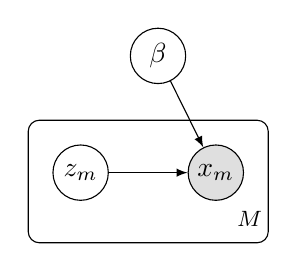
\begin{tikzpicture}

  % Nodes
  \node[latent]               (beta)      {$\beta$} ;
  \node[left=0.5cm of beta]               (betaph)      {} ;
  \node[latent, below=1.0cm of betaph] (z)    {$z_m$} ;
  \node[obs, right=1.0cm of z]      (x)        {$x_m$} ;

  % Edges
  % \edge{beta}{z};
  \edge{beta}{x};
  \edge{z}{x};

  % Plates
  \plate[inner sep=0.3cm,
    label={[xshift=-15pt,yshift=15pt]south east:$M$}] {plate1} {
    (x)(z)
  } {};

\end{tikzpicture}

\caption{Data subsampling with a hierarchical model. We define
a subgraph of the full model, forming a plate of size $M$ rather than
$N$.}
\end{figure}

In the subgraph setting, we do data subsampling while working with a
subgraph of the full model. This setting is necessary when the data
and model do not fit in memory.
It is scalable in that both the
algorithm's computational complexity (per iteration) and memory
complexity are independent of the data set size.

For example, consider a hierarchical model,
\begin{equation*}
p(\mathbf{x}, \mathbf{z}, \beta)
= p(\beta) \prod_{n=1}^N p(z_n \mid \beta) p(x_n \mid z_n, \beta),
\end{equation*}
where there are latent variables $z_n$ for
each data point $x_n$ (local variables) and latent variables $\beta$
which are shared across data points (global variables).

To avoid memory issues, we work on only a subgraph of the model,
\begin{equation*}
p(\mathbf{x}, \mathbf{z}, \beta)
= p(\beta) \prod_{m=1}^M p(z_m \mid \beta) p(x_m \mid z_m, \beta).
\end{equation*}
More concretely, we define a mixture of Gaussians over
$D$-dimensional data $\{x_n\}\in\mathbb{R}^{N\times D}$. There are $K$
latent cluster means $\{\beta_k\}\in\mathbb{R}^{K\times D}$ and a
membership assignment $z_n\in\{0,\ldots,K-1\}$ for each data point
$x_n$.

\begin{lstlisting}[language=Python]
N = 10000000  # data set size
M = 128  # minibatch size
D = 2  # data dimensionality
K = 5  # number of clusters

beta = Normal(mu=tf.zeros([K, D]), sigma=tf.ones([K, D]))
z = Categorical(logits=tf.zeros([M, K]))
x = Normal(mu=tf.gather(beta, z), sigma=tf.ones([M, D]))
\end{lstlisting}

For inference, the variational model is
\begin{equation*}
q(\mathbf{z}, \beta) =
q(\beta; \lambda) \prod_{n=1}^N q(z_n \mid \beta; \gamma_n),
\end{equation*}
parameterized by $\{\lambda, \{\gamma_n\}\}$.
Again, we work on only a subgraph of the model,
\begin{equation*}
q(\mathbf{z}, \beta) =
q(\beta; \lambda) \prod_{m=1}^M q(z_m \mid \beta; \gamma_m).
\end{equation*}
parameterized by $\{\lambda, \{\gamma_m\}\}$. Importantly, only $M$
parameters are stored in memory for $\{\gamma_m\}$ rather than $N$.

\begin{lstlisting}[language=Python]
qbeta = Normal(mu=tf.Variable(tf.zeros([K, D])),
               sigma=tf.nn.softplus(tf.Variable(tf.zeros[K, D])))
qz_variables = tf.Variable(tf.zeros([M, K]))
qz = Categorical(logits=qz_variables)
\end{lstlisting}

We will perform inference with \texttt{KLqp}, a variational method
that minimizes the divergence measure $\text{KL}(q\| p)$.

We instantiate two algorithms: a global inference over $\beta$ given
the subset of $\mathbf{z}$ and a local inference over the subset of
$\mathbf{z}$ given $\beta$.
We also pass in a TensorFlow placeholder \texttt{x_ph} for the data,
so we can change the data at each step. (Alternatively,
{batch tensors} can be used.)

\begin{lstlisting}[language=Python]
x_ph = tf.placeholder(tf.float32, [M])
inference_global = ed.KLqp({beta: qbeta}, data={x: x_ph, z: qz})
inference_local = ed.KLqp({z: qz}, data={x: x_ph, beta: qbeta})
\end{lstlisting}

We initialize the algorithms with the \texttt{scale} argument, so that
computation on \texttt{z} and \texttt{x} will be scaled appropriately.
This enables unbiased estimates for stochastic gradients.

\begin{lstlisting}[language=Python]
inference_global.initialize(scale={x: float(N) / M, z: float(N) / M})
inference_local.initialize(scale={x: float(N) / M, z: float(N) / M})
\end{lstlisting}

Conceptually, the scale argument represents scaling for each random
variable’s plate, as if we had seen that random variable $N/M$ as many
times.

We now run inference, assuming there is a \texttt{next_batch} function
which provides the next batch of data.

\begin{lstlisting}[language=Python]
qz_init = tf.initialize_variables([qz_variables])
for _ in range(1000):
  x_batch = next_batch(size=M)
  for _ in range(10):  # make local inferences
    inference_local.update(feed_dict={x_ph: x_batch})

  # update global parameters
  inference_global.update(feed_dict={x_ph: x_batch})
  # reinitialize the local factors
  qz_init.run()
\end{lstlisting}

After each iteration, we also reinitialize the parameters for
$q(\mathbf{z}\mid\beta)$; this is because we do inference on a new
set of local variational factors for each batch.

This demo readily applies to other inference algorithms such as
\texttt{SGLD} (stochastic gradient Langevin dynamics): simply
replace \texttt{qbeta} and \texttt{qz} with \texttt{Empirical} random
variables; then call \texttt{ed.SGLD} instead of \texttt{ed.KLqp}.

\subsubsection{Advanced settings}

If the parameters fit in memory, one can avoid having to reinitialize
local parameters or read/write from disk.  To do this, define the full
set of parameters and index them into the local posterior factors.

\begin{lstlisting}[language=Python]
qz_variables = tf.Variable(tf.zeros([N, K]))
idx_ph = tf.placeholder(tf.int32, [M])
qz = Categorical(logits=tf.gather(qz_variables, idx_ph))
\end{lstlisting}

We define an index placeholder \texttt{idx_ph}. It will be fed index
values at runtime to determine which parameters correspond to a given
data subsample.
% As an example, see the script for
% \href{https://github.com/blei-lab/edward/blob/master/examples/probabilistic_pca_subsampling.py}
% {probabilistic principal components analysis} with stochastic
% variational inference.

An alternative approach to reduce memory complexity is to use an
inference network \citep{dayan1995helmholtz}, also known as
amortized inference \citep{stuhlmuller2013learning}.  This can be
applied using a global parameterization of $q(\mathbf{z}, \beta)$.
% For more details, see the
% \href{/tutorials/inference-networks}{inference networks tutorial}.

In streaming data, or online inference, the size of the data $N$
may be unknown, or conceptually the size of the data may be
infinite and at any time in which we query parameters from the online
algorithm, the outputted parameters are from having processed as many
data points up to that time.
The approach of Bayesian filtering
\citep{doucet2000on,broderick2013streaming} can be applied in Edward using
recursive posterior inferences; the approach of population posteriors
\citep{mcinerney2015population} is readily applicable from the subgraph
setting.

In other settings, working on a subgraph of the model does not
apply, such as in time series models when we want to
preserve dependencies across time steps in our variational model.
Approaches in the literature can be applied in Edward
\citep{binder1997space,johnson2014stochastic,foti2014stochastic}.

\subsubsection*{Development of Inference Methods}

Edward uses class inheritance to provide a hierarchy of inference
methods. This enables fast experimentation on top of existing
algorithms, whether it be developing new black box algorithms or
new model-specific algorithms.

\begin{figure}[!htb]
\centering
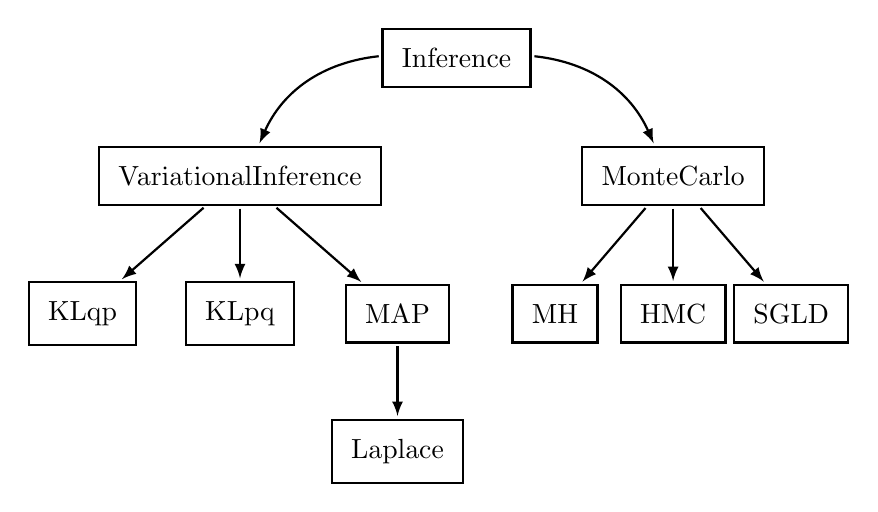
\begin{tikzpicture}
    \begin{pgfonlayer}{nodelayer}
        \node [style=box] (0) at (2.25, 2) {Inference};
        \node [style=box] (1) at (-0.5, 0.5) {VariationalInference};
        \node [style=box] (2) at (5, 0.5) {MonteCarlo};
        \node [style=box] (3) at (-2.5, -1.25) {KLqp};
        \node [style=box] (4) at (-0.5, -1.25) {KLpq};
        \node [style=box] (5) at (1.5, -1.25) {MAP};
        \node [style=box] (6) at (1.5, -3) {Laplace};
        % \node [style=box] (7) at (4.0, -1.25) {GANInference};
        % \node [style=box] (8) at (4.0, -3) {WGANInference};
        \node [style=box] (9) at (3.5, -1.25) {MH};
        \node [style=box] (10) at (5, -1.25) {HMC};
        \node [style=box] (11) at (6.5, -1.25) {SGLD};
        % \node [style=box] (10) at (7.5, 0.5) {Exact};
        %\node [style=box] (10) at (-4, -1.25) {CollapsedInference};
        %\node [style=box] (11) at (-5, -1.25) {ConjugateInference};
    \end{pgfonlayer}
    \begin{pgfonlayer}{edgelayer}
        \draw [style=arrow, bend right] (0) to (1);
        \draw [style=arrow] (1) to (3);
        \draw [style=arrow] (1) to (4);
        \draw [style=arrow] (1) to (5);
        \draw [style=arrow] (5) to (6);
        % \draw [style=arrow] (1) to (7);
        % \draw [style=arrow] (7) to (8);
        \draw [style=arrow, bend left] (0) to (2);
        %\draw [style=arrow, bend left, draw=Gray] (0) to (2);
        \draw [style=arrow] (2) to (9);
        \draw [style=arrow] (2) to (10);
        \draw [style=arrow] (2) to (11);
        % \draw [style=arrow, bend left, out=17] (0) to (10);
        %\draw [style=arrow] (9) to (10);
        %\draw [style=arrow] (9) to (11);
    \end{pgfonlayer}
\end{tikzpicture}

\caption{Dependency graph of several inference methods. Nodes are classes in Edward
and arrows represent class inheritance.}
\end{figure}

There is a base class \texttt{Inference}, from which all inference
methods are derived from. Note that \texttt{Inference} says nothing
about the class of models that an algorithm must work with. One can
build inference algorithms which are tailored to a restricted class of
models available in Edward (such as differentiable models or
conditionally conjugate models), or even tailor it to a single model.
The algorithm can raise an error if the model is outside this class.

We organize inference under two paradigms:
\texttt{VariationalInference} and \texttt{MonteCarlo} (or more plainly,
optimization and sampling). These inherit from \texttt{Inference} and each
have their own default methods.

For example, developing a new variational inference algorithm is as simple as
inheriting from \texttt{VariationalInference} and writing a
\texttt{build_loss_and_gradients()} method. \texttt{VariationalInference} implements many default methods such
as \texttt{initialize()} with options for an optimizer.
For example, see the
importance weighted variational inference
script.%
\footnote{\url{https://github.com/blei-lab/edward/blob/master/examples/iwvi.py}}

\subsection{Criticism}

We can never validate whether a model is true. In practice, ``all
models are wrong'' \citep{box1976science}. However, we can try to
uncover where the model goes wrong. Model criticism helps justify the
model as an approximation or point to good directions for revising the
model.

Edward explores model criticism using
\begin{itemize}
  \item point-based evaluations, such as mean squared error or
  classification accuracy;
  \item posterior predictive checks, for making probabilistic
  assessments of the model fit using discrepancy functions.
\end{itemize}

We describe them in detail below.

\subsubsection{Point-based evaluations}

A point-based evaluation is a scalar-valued metric for assessing
trained models \citep{winkler1996scoring,gneiting2007strictly}.
For example, we can assess models for classification
by predicting the label for each observation in the data and comparing
it to their true labels. Edward implements a variety of metrics, such
as classification error and mean absolute error.

Formally, point prediction in probabilistic models is given by
taking the mean of the posterior predictive distribution,
\begin{align*}
  p(\mathbf{x}_\text{new} \mid \mathbf{x})
  &=
  \int
  p(\mathbf{x}_\text{new} \mid \mathbf{z})
  p(\mathbf{z} \mid \mathbf{x})
  \text{d} \mathbf{z}.
\end{align*}
The model's posterior predictive can be used to generate new data
given past observations and can also make predictions on new data
given past observations.
It is formed by calculating the likelihood of the new data, averaged
over every set of latent variables according to the posterior
distribution.

\subsubsection{Implementation}

To evaluate inferred models, we first form the posterior
predictive distribution. A helpful utility function for this is
\texttt{copy}. For example,
assume the model defines a likelihood \texttt{x} connected to a prior
\texttt{z}. The posterior predictive distribution is
\begin{lstlisting}[language=Python]
x_post = ed.copy(x, {z: qz})
\end{lstlisting}
Here, we copy the likelihood node \texttt{x} in the graph and replace dependence
on the prior \texttt{z} with dependence on the inferred posterior \texttt{qz}.

The \texttt{ed.evaluate()} method takes as input a set of metrics to
evaluate, and a data dictionary. As with inference, the data dictionary binds the
observed random variables in the model to realizations: in this case,
it is the posterior predictive random variable of outputs \texttt{y_post} to
\texttt{y_train} and a placeholder for inputs \texttt{x} to
\texttt{x_train}.
\begin{lstlisting}[language=Python]
ed.evaluate('categorical_accuracy', data={y_post: y_train, x: x_train})
ed.evaluate('mean_absolute_error', data={y_post: y_train, x: x_train})
\end{lstlisting}
The \texttt{data} can be data held-out from training time, making it
easy to implement cross-validated techniques.

Point-based evaluation applies generally to any setting, including
unsupervised tasks. For example, we can evaluate the likelihood of
observing the data.
\begin{lstlisting}[language=Python]
ed.evaluate('log_likelihood', data={x_post: x_train})
\end{lstlisting}

It is common practice to criticize models with data held-out from
training. To do this, we first perform inference over any local latent
variables of the held-out data, fixing the global variables.  Then we
make predictions on the held-out data.

\begin{lstlisting}[language=Python]
from edward.models import Categorical

# create local posterior factors for test data, assuming test data
# has N_test many data points
qz_test = Categorical(logits=tf.Variable(tf.zeros[N_test, K]))

# run local inference conditional on global factors
inference_test = ed.Inference({z: qz_test}, data={x: x_test, beta: qbeta})
inference_test.run()

# build posterior predictive on test data
x_post = ed.copy(x, {z: qz_test, beta: qbeta}})
ed.evaluate('log_likelihood', data={x_post: x_test})
\end{lstlisting}

Point-based evaluations are formally known as scoring rules
in decision theory. Scoring rules are useful for model comparison, model
selection, and model averaging.

\subsubsection{Posterior predictive checks}

Posterior predictive checks (PPCs)
analyze the degree to which data generated from the model deviate from
data generated from the true distribution. They can be used either
numerically to quantify this degree, or graphically to visualize this
degree. PPCs can be thought of as a probabilistic generalization of
point-based evaluations
\citep{box1980sampling,rubin1984bayesianly,meng1994posterior,gelman1996posterior}.

PPCs focus on the posterior predictive distribution
\begin{align*}
  p(\mathbf{x}_\text{new} \mid \mathbf{x})
  &=
  \int
  p(\mathbf{x}_\text{new} \mid \mathbf{z})
  p(\mathbf{z} \mid \mathbf{x})
  \text{d} \mathbf{z}.
\end{align*}
% The model's posterior predictive can be used to generate new data
% given past observations and can also make predictions on new data
% given past observations.
% It is formed by calculating the likelihood of the new data, averaged
% over every set of latent variables according to the posterior
% distribution.
%
The simplest PPC works by applying a test statistic on new data
generated from the posterior predictive, such as
$T(\mathbf{x}_\text{new}) = \max(\mathbf{x}_\text{new})$.  Applying
$T(\mathbf{x}_\text{new})$ to new data over many data replications
induces a distribution. We compare this distribution to the test
statistic applied to the real data $T(\mathbf{x})$.

% \includegraphics{/images/ppc.png}

In the figure, $T(\mathbf{x})$ falls in a low probability region of
this reference distribution. This indicates that the model fits the
data poorly according to this check; this suggests an area of
improvement for the model.

More generally, the test statistic can also be a function of the
model's latent variables $T(\mathbf{x}, \mathbf{z})$, known as a
discrepancy function.  Examples of discrepancy functions are the
metrics used for point-based evaluation. We can now interpret the
point-based evaluation as a special case of PPCs: it simply calculates
$T(\mathbf{x}, \mathbf{z})$ over the real data and without a reference
distribution in mind. A reference distribution allows us to make
probabilistic statements about the point, in reference to an overall
distribution.

\subsubsection{Implementation}

To evaluate inferred models, we first form the posterior
predictive distribution. A helpful utility function for this is
\texttt{copy}. For example,
assume the model defines a likelihood \texttt{x} connected to a prior
\texttt{z}. The posterior predictive distribution is
\begin{lstlisting}[language=Python]
x_post = ed.copy(x, {z: qz})
\end{lstlisting}
Here, we copy the likelihood node \texttt{x} in the graph and replace dependence
on the prior \texttt{z} with dependence on the inferred posterior \texttt{qz}.

The \texttt{ed.ppc()} method provides a scaffold for studying
various discrepancy functions.
\begin{lstlisting}[language=Python]
def T(xs, zs):
  return tf.reduce_mean(xs[x_post])

ed.ppc(T, data={x_post: x_train})
\end{lstlisting}
The discrepancy can also take latent variables as input, which we pass
into the PPC.
\begin{lstlisting}[language=Python]
def T(xs, zs):
  return tf.reduce_mean(tf.cast(zs['z'], tf.float32))

ppc(T, data={y_post: y_train, x_ph: x_train},
    latent_vars={'z': qz, 'beta': qbeta})
\end{lstlisting}

% See the \href{/api/criticism}{criticism API} for further details.

PPCs are an excellent tool for revising models, simplifying or
expanding the current model as one examines how well it fits the data.
They are inspired by prior checks and classical hypothesis
testing, under the philosophy that models should be
criticized under the frequentist perspective of large sample
assessment.

PPCs can also be applied to tasks such as hypothesis testing, model
comparison, model selection, and model averaging.  It's important to
note that while they can be applied as a form of Bayesian hypothesis
testing, hypothesis testing is generally not recommended: binary
decision making from a single test is not as common a use case as one
might believe. We recommend performing many PPCs to get a holistic
understanding of the model fit.

\clearpage
\section{End-to-end Examples}
\label{sec:examples}

\subsection{Bayesian Linear Regression}

In supervised learning, the task is to infer hidden structure from
labeled data, comprised of training examples $\{(x_n, y_n)\}$.
Regression (typically) means the output $y$ takes continuous values.

\subsubsection{Data}

Simulate training and test sets of $500$ data points. They comprise
pairs of inputs $\mathbf{x}_n\in\mathbb{R}^{5}$ and outputs
$y_n\in\mathbb{R}$. They have a linear dependence of
\begin{align*}
  \mathbf{w}_{\text{true}}
  &=
  (-1.25, 4.51, 2.32, 0.99, -3.44).
\end{align*}
with normally distributed noise.

\begin{lstlisting}
def build_toy_dataset(N, w, noise_std=0.1):
  D = len(w)
  x = np.random.randn(N, D).astype(np.float32)
  y = np.dot(x, w) + np.random.normal(0, noise_std, size=N)
  return x, y

N = 500  # number of  data points
D = 5  # number of  features

w_true = 10 * (np.random.rand(D) - 0.5)
X_train, y_train = build_toy_dataset(N, w_true)
X_test, y_test = build_toy_dataset(N, w_true)
\end{lstlisting}

\subsubsection{Model}

Posit the model as Bayesian linear regression. It relates
outputs $y\in\mathbb{R}$, also known as the response, given
a vector of inputs
$\mathbf{x}\in\mathbb{R}^D$, also known as the features or covariates.
The model assumes a
linear relationship between these two random variables
\citep{murphy2012machine}.

For a set of $N$ data points $(\mathbf{X},\mathbf{y})=\{(\mathbf{x}_n, y_n)\}$,
the model posits the following conditional relationships:
\begin{align*}
  p(\mathbf{w})
  &=
  \text{Normal}(\mathbf{w} \mid \mathbf{0}, \sigma_w^2\mathbf{I}),
  \\[1.5ex]
  p(b)
  &=
  \text{Normal}(b \mid 0, \sigma_b^2),
  \\
  p(\mathbf{y} \mid \mathbf{w}, b, \mathbf{X})
  &=
  \prod_{n=1}^N
  \text{Normal}(y_n \mid \mathbf{x}_n^\top\mathbf{w} + b, \sigma_y^2).
\end{align*}
The latent variables are the linear model's weights $\mathbf{w}$ and
intercept $b$, also known as the bias.
Assume $\sigma_w^2,\sigma_b^2$ are known prior variances and $\sigma_y^2$ is a
known likelihood variance. The mean of the likelihood is given by a
linear transformation of the inputs $\mathbf{x}_n$.

\begin{lstlisting}
X = tf.placeholder(tf.float32, [N, D])
w = Normal(mu=tf.zeros(D), sigma=tf.ones(D))
b = Normal(mu=tf.zeros(1), sigma=tf.ones(1))
y = Normal(mu=ed.dot(X, w) + b, sigma=tf.ones(N))
\end{lstlisting}

\subsubsection{Inference}

We now turn to inferring the posterior using variational inference.
Define the variational model to be a fully factorized normal across
the weights.
\begin{lstlisting}
qw = Normal(mu=tf.Variable(tf.random_normal([D])),
            sigma=tf.nn.softplus(tf.Variable(tf.random_normal([D]))))
qb = Normal(mu=tf.Variable(tf.random_normal([1])),
            sigma=tf.nn.softplus(tf.Variable(tf.random_normal([1]))))
\end{lstlisting}

Run variational inference with the Kullback-Leibler divergence, using a
default of $1000$ iterations.
\begin{lstlisting}
inference = ed.KLqp({w: qw, b: qb}, data={X: X_train, y: y_train})
inference.run()
\end{lstlisting}
In this case \texttt{KLqp} defaults to minimizing the
$\text{KL}(q\|p)$ divergence measure using the reparameterization
gradient.
Minimizing this divergence metric is equivalent to maximizing the
evidence lower bound (\textsc{elbo}). Figure\nobreakspace \ref{fig:supervised-elbo} shows the
progression of the \textsc{elbo} across iterations; variational inference
appears to converge in approximately 200 iterations.

\begin{figure}[htb]
\centering
% This file was created by matplotlib2tikz v0.5.15.
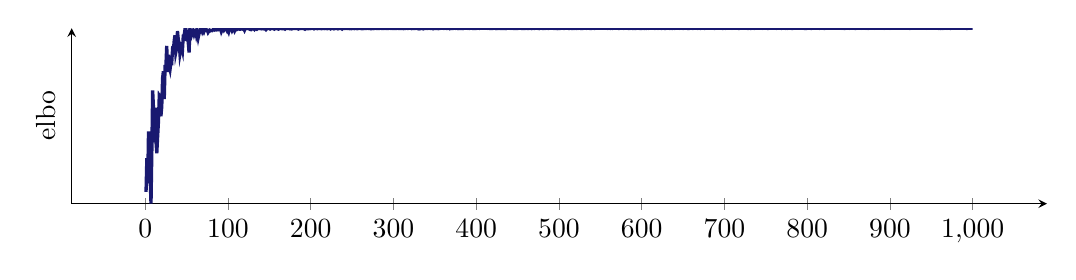
\begin{tikzpicture}

\begin{axis}[
width=5.5in,
height=1.5in,
axis lines=left,
enlarge x limits=0.09,
ylabel={\textsc{elbo}},
ylabel near ticks,
ytick=\empty,
% legend entries={{$\textsc{elbo}$}},
% legend style={draw=none, at={(1.0,1.0)}, anchor=north east,font=\small},
% legend cell align=left,
]
\addplot [very thick, MidnightBlue]
table {%
1 -24832.922
2 -19803.498
3 -23561.203
4 -15824.293
5 -20963.410
6 -22910.539
7 -26589.451
8 -18808.270
9 -9747.762
10 -12387.727
11 -17470.422
12 -12321.565
13 -17315.900
14 -19084.033
15 -16630.318
16 -14351.264
17 -10512.238
18 -10711.228
19 -13574.313
20 -12119.984
21 -7890.950
22 -6892.946
23 -11034.027
24 -6176.863
25 -6172.959
26 -3107.659
27 -7020.251
28 -4452.798
29 -6089.138
30 -6615.671
31 -5675.927
32 -5712.329
33 -3730.986
34 -3880.640
35 -2384.833
36 -1533.137
37 -4068.863
38 -3454.978
39 -919.619
40 -2226.556
41 -2632.443
42 -4297.725
43 -3595.808
44 -3212.551
45 -3748.414
46 -1623.859
47 -1570.649
48 -740.249
49 -2372.888
50 -1205.361
51 -1917.089
52 -2547.169
53 -4118.985
54 -621.050
55 -757.427
56 -1556.877
57 -1209.368
58 -889.026
59 -1362.566
60 -966.671
61 -845.125
62 -1561.782
63 -1137.697
64 -1877.333
65 -1303.988
66 -1014.029
67 -591.169
68 -611.487
69 -991.204
70 -681.929
71 -984.964
72 -658.884
73 -763.687
74 -714.870
75 -763.138
76 -1100.189
77 -909.522
78 -784.309
79 -874.663
80 -824.489
81 -841.660
82 -717.680
83 -575.089
84 -705.678
85 -583.816
86 -738.280
87 -730.617
88 -509.557
89 -653.959
90 -559.539
91 -562.100
92 -984.054
93 -689.061
94 -538.112
95 -761.587
96 -533.470
97 -559.037
98 -589.960
99 -838.655
100 -584.534
101 -962.970
102 -518.553
103 -612.928
104 -522.122
105 -845.492
106 -619.405
107 -576.229
108 -865.849
109 -589.953
110 -508.640
111 -669.911
112 -607.241
113 -560.890
114 -629.296
115 -626.430
116 -568.982
117 -605.701
118 -629.469
119 -537.192
120 -781.661
121 -500.954
122 -540.029
123 -535.272
124 -529.918
125 -578.479
126 -601.557
127 -682.052
128 -701.809
129 -529.723
130 -532.800
131 -542.383
132 -670.603
133 -499.615
134 -529.973
135 -633.945
136 -542.460
137 -530.477
138 -531.029
139 -548.708
140 -503.343
141 -576.710
142 -550.642
143 -573.576
144 -599.329
145 -514.116
146 -676.929
147 -520.751
148 -549.704
149 -519.155
150 -532.308
151 -606.272
152 -529.381
153 -521.502
154 -515.503
155 -566.671
156 -627.266
157 -519.156
158 -505.319
159 -548.680
160 -574.648
161 -624.666
162 -565.911
163 -527.196
164 -516.848
165 -555.894
166 -555.441
167 -552.636
168 -533.432
169 -616.256
170 -514.473
171 -515.411
172 -521.036
173 -542.845
174 -538.216
175 -580.167
176 -550.768
177 -594.729
178 -550.794
179 -519.260
180 -524.028
181 -539.773
182 -536.005
183 -500.866
184 -503.364
185 -594.558
186 -507.863
187 -545.172
188 -514.240
189 -505.776
190 -533.364
191 -512.997
192 -563.213
193 -631.401
194 -531.153
195 -554.997
196 -543.574
197 -572.771
198 -549.754
199 -526.739
200 -545.172
201 -499.916
202 -499.685
203 -518.962
204 -577.682
205 -516.530
206 -507.992
207 -502.159
208 -558.325
209 -527.241
210 -501.722
211 -530.918
212 -531.191
213 -565.879
214 -506.361
215 -509.624
216 -507.127
217 -544.332
218 -507.483
219 -526.420
220 -562.512
221 -530.384
222 -518.334
223 -506.957
224 -583.284
225 -501.156
226 -521.283
227 -522.312
228 -580.823
229 -530.023
230 -522.596
231 -530.254
232 -501.868
233 -575.415
234 -521.655
235 -500.199
236 -534.586
237 -503.783
238 -601.045
239 -501.512
240 -530.466
241 -518.048
242 -510.544
243 -491.884
244 -524.739
245 -505.006
246 -534.611
247 -549.057
248 -499.555
249 -556.432
250 -526.919
251 -533.946
252 -506.801
253 -546.932
254 -512.135
255 -495.986
256 -556.187
257 -507.510
258 -511.102
259 -502.828
260 -513.216
261 -508.672
262 -558.700
263 -527.179
264 -543.484
265 -506.969
266 -532.850
267 -506.210
268 -516.335
269 -495.212
270 -517.379
271 -528.253
272 -497.483
273 -572.889
274 -546.855
275 -498.365
276 -543.458
277 -518.540
278 -493.510
279 -517.002
280 -536.921
281 -509.926
282 -525.150
283 -520.514
284 -500.861
285 -506.285
286 -520.448
287 -505.468
288 -514.473
289 -510.371
290 -501.895
291 -517.209
292 -518.540
293 -522.171
294 -527.152
295 -498.954
296 -497.152
297 -523.719
298 -496.689
299 -520.748
300 -518.319
301 -524.671
302 -510.265
303 -510.676
304 -508.489
305 -497.077
306 -526.555
307 -520.639
308 -517.420
309 -523.865
310 -537.216
311 -503.112
312 -544.220
313 -510.059
314 -521.773
315 -505.111
316 -503.992
317 -524.134
318 -512.138
319 -498.316
320 -504.593
321 -499.354
322 -546.580
323 -514.315
324 -515.279
325 -512.180
326 -517.124
327 -506.894
328 -494.740
329 -533.814
330 -569.474
331 -502.172
332 -571.643
333 -513.843
334 -510.310
335 -503.516
336 -575.851
337 -504.016
338 -534.706
339 -497.825
340 -512.104
341 -518.426
342 -503.748
343 -509.475
344 -499.075
345 -533.529
346 -504.493
347 -500.657
348 -567.336
349 -532.630
350 -514.995
351 -526.937
352 -513.165
353 -531.044
354 -550.746
355 -504.847
356 -521.411
357 -498.129
358 -508.284
359 -506.762
360 -506.213
361 -512.521
362 -499.582
363 -501.453
364 -519.875
365 -511.799
366 -495.873
367 -506.501
368 -565.908
369 -509.649
370 -515.521
371 -526.465
372 -518.555
373 -502.669
374 -504.838
375 -509.898
376 -504.504
377 -510.423
378 -542.953
379 -504.786
380 -526.260
381 -521.690
382 -531.245
383 -516.041
384 -540.712
385 -504.336
386 -504.113
387 -502.955
388 -501.416
389 -497.498
390 -514.521
391 -500.098
392 -515.770
393 -499.772
394 -508.010
395 -507.638
396 -520.820
397 -529.995
398 -510.079
399 -524.253
400 -514.175
401 -502.353
402 -508.909
403 -504.541
404 -512.921
405 -504.037
406 -499.760
407 -503.540
408 -506.858
409 -499.937
410 -498.388
411 -499.468
412 -498.646
413 -505.261
414 -508.928
415 -503.252
416 -519.530
417 -510.247
418 -510.240
419 -523.058
420 -519.503
421 -500.548
422 -506.653
423 -502.075
424 -546.387
425 -530.292
426 -540.231
427 -499.338
428 -506.619
429 -515.662
430 -529.709
431 -529.118
432 -508.514
433 -523.447
434 -517.518
435 -501.008
436 -537.748
437 -501.082
438 -504.598
439 -503.611
440 -500.672
441 -510.425
442 -499.719
443 -511.103
444 -505.230
445 -511.932
446 -500.884
447 -539.216
448 -529.175
449 -537.471
450 -524.694
451 -502.843
452 -496.148
453 -506.900
454 -507.648
455 -509.699
456 -520.198
457 -519.453
458 -506.753
459 -518.399
460 -495.285
461 -505.901
462 -522.508
463 -527.759
464 -508.374
465 -504.670
466 -503.456
467 -539.282
468 -496.581
469 -500.324
470 -515.431
471 -508.935
472 -501.346
473 -497.972
474 -500.478
475 -521.828
476 -542.320
477 -506.258
478 -495.614
479 -505.659
480 -514.763
481 -512.574
482 -516.924
483 -497.719
484 -512.537
485 -496.289
486 -503.220
487 -519.888
488 -510.391
489 -496.645
490 -501.112
491 -507.252
492 -503.251
493 -496.841
494 -518.408
495 -503.256
496 -510.145
497 -508.684
498 -541.055
499 -510.272
500 -508.380
501 -526.208
502 -505.449
503 -508.021
504 -501.584
505 -496.387
506 -517.301
507 -506.702
508 -501.748
509 -500.537
510 -496.489
511 -507.099
512 -513.221
513 -514.784
514 -494.533
515 -511.332
516 -506.822
517 -524.429
518 -496.344
519 -510.229
520 -501.417
521 -520.455
522 -499.426
523 -511.695
524 -504.585
525 -503.283
526 -511.264
527 -515.652
528 -509.630
529 -511.151
530 -506.625
531 -505.202
532 -497.890
533 -510.685
534 -506.627
535 -507.428
536 -504.274
537 -509.759
538 -522.179
539 -523.910
540 -504.896
541 -502.109
542 -506.130
543 -517.468
544 -500.137
545 -498.487
546 -501.097
547 -500.590
548 -507.752
549 -499.834
550 -502.212
551 -504.722
552 -500.224
553 -504.556
554 -504.306
555 -503.422
556 -502.557
557 -498.314
558 -505.328
559 -510.563
560 -504.654
561 -499.723
562 -516.698
563 -501.232
564 -508.030
565 -510.750
566 -500.261
567 -498.932
568 -502.426
569 -505.373
570 -498.250
571 -503.679
572 -514.284
573 -512.353
574 -499.591
575 -499.622
576 -502.963
577 -496.011
578 -511.305
579 -506.990
580 -500.962
581 -503.827
582 -501.354
583 -500.075
584 -515.265
585 -504.798
586 -513.242
587 -498.378
588 -497.362
589 -516.766
590 -510.508
591 -502.276
592 -523.989
593 -513.169
594 -499.786
595 -497.028
596 -508.840
597 -505.038
598 -516.705
599 -510.934
600 -516.177
601 -503.793
602 -500.364
603 -517.858
604 -502.610
605 -511.523
606 -510.420
607 -498.120
608 -511.895
609 -498.941
610 -497.207
611 -500.341
612 -507.238
613 -498.622
614 -499.937
615 -504.822
616 -513.693
617 -503.950
618 -503.808
619 -507.735
620 -510.914
621 -496.255
622 -499.346
623 -503.904
624 -519.045
625 -500.680
626 -506.674
627 -504.924
628 -523.276
629 -515.196
630 -503.100
631 -506.020
632 -497.345
633 -502.293
634 -517.487
635 -497.628
636 -506.710
637 -515.729
638 -500.366
639 -500.153
640 -512.040
641 -498.316
642 -502.173
643 -504.783
644 -501.223
645 -500.492
646 -509.528
647 -498.987
648 -502.461
649 -502.459
650 -511.940
651 -505.319
652 -502.409
653 -501.323
654 -507.214
655 -499.913
656 -530.570
657 -512.025
658 -508.064
659 -503.212
660 -499.930
661 -505.267
662 -514.629
663 -500.950
664 -505.419
665 -505.696
666 -497.856
667 -508.020
668 -510.515
669 -502.513
670 -503.230
671 -515.594
672 -496.592
673 -503.725
674 -500.498
675 -499.564
676 -516.964
677 -503.196
678 -505.050
679 -500.136
680 -499.966
681 -496.349
682 -506.102
683 -500.523
684 -500.489
685 -506.254
686 -500.197
687 -501.952
688 -519.274
689 -499.919
690 -503.175
691 -504.537
692 -499.757
693 -502.693
694 -498.425
695 -502.422
696 -504.033
697 -503.499
698 -517.570
699 -505.387
700 -500.494
701 -509.516
702 -507.658
703 -503.182
704 -506.818
705 -498.547
706 -496.710
707 -501.242
708 -499.315
709 -509.116
710 -497.264
711 -499.059
712 -498.797
713 -497.495
714 -508.322
715 -506.021
716 -505.151
717 -512.350
718 -509.821
719 -501.822
720 -500.342
721 -495.944
722 -501.319
723 -502.265
724 -501.476
725 -503.717
726 -504.835
727 -498.007
728 -511.145
729 -512.207
730 -495.707
731 -505.319
732 -517.518
733 -500.396
734 -498.152
735 -496.250
736 -511.999
737 -502.275
738 -500.993
739 -501.565
740 -502.559
741 -502.758
742 -499.287
743 -504.771
744 -497.680
745 -501.568
746 -508.972
747 -501.550
748 -499.927
749 -506.345
750 -505.651
751 -505.419
752 -510.120
753 -510.091
754 -503.827
755 -495.517
756 -504.425
757 -508.215
758 -503.453
759 -500.999
760 -499.582
761 -494.836
762 -494.701
763 -510.070
764 -506.157
765 -505.592
766 -503.926
767 -496.379
768 -505.495
769 -513.070
770 -501.799
771 -499.353
772 -503.395
773 -495.691
774 -512.763
775 -503.920
776 -509.860
777 -504.101
778 -501.568
779 -504.793
780 -507.061
781 -507.604
782 -526.716
783 -506.790
784 -498.373
785 -499.975
786 -507.128
787 -504.331
788 -498.521
789 -500.208
790 -502.291
791 -505.092
792 -501.648
793 -504.965
794 -499.602
795 -498.995
796 -506.491
797 -517.031
798 -502.801
799 -520.839
800 -505.293
801 -500.011
802 -500.577
803 -499.595
804 -501.668
805 -519.901
806 -501.038
807 -498.892
808 -500.228
809 -506.250
810 -499.398
811 -504.560
812 -497.615
813 -499.576
814 -501.447
815 -511.313
816 -496.942
817 -505.703
818 -499.415
819 -505.719
820 -508.774
821 -516.705
822 -498.311
823 -496.940
824 -503.315
825 -498.452
826 -503.590
827 -496.700
828 -505.269
829 -497.584
830 -497.001
831 -503.100
832 -500.741
833 -497.989
834 -500.802
835 -507.409
836 -498.523
837 -495.966
838 -501.295
839 -505.662
840 -504.811
841 -499.122
842 -508.961
843 -503.303
844 -504.203
845 -519.745
846 -510.439
847 -500.487
848 -501.894
849 -499.687
850 -501.675
851 -508.799
852 -498.292
853 -502.280
854 -501.178
855 -500.300
856 -500.580
857 -508.458
858 -508.773
859 -508.863
860 -500.323
861 -499.661
862 -507.355
863 -500.921
864 -503.958
865 -502.179
866 -508.534
867 -501.389
868 -503.068
869 -500.272
870 -501.099
871 -508.925
872 -495.506
873 -508.646
874 -509.754
875 -497.287
876 -500.348
877 -498.079
878 -507.489
879 -497.506
880 -502.639
881 -508.541
882 -506.465
883 -500.146
884 -498.308
885 -496.296
886 -501.985
887 -497.248
888 -503.042
889 -497.521
890 -498.882
891 -497.171
892 -499.977
893 -510.504
894 -500.521
895 -508.016
896 -507.364
897 -500.553
898 -503.865
899 -503.870
900 -508.329
901 -496.506
902 -503.336
903 -498.970
904 -504.545
905 -500.459
906 -499.504
907 -500.112
908 -499.521
909 -502.887
910 -498.618
911 -499.378
912 -497.413
913 -497.134
914 -501.098
915 -496.958
916 -501.820
917 -502.435
918 -504.083
919 -496.351
920 -496.450
921 -501.246
922 -498.509
923 -498.536
924 -514.812
925 -501.555
926 -500.779
927 -499.724
928 -499.486
929 -500.125
930 -503.387
931 -499.596
932 -498.748
933 -498.041
934 -506.005
935 -501.958
936 -504.011
937 -506.678
938 -502.875
939 -502.559
940 -503.202
941 -506.613
942 -501.716
943 -504.522
944 -508.776
945 -503.441
946 -495.678
947 -502.650
948 -496.957
949 -499.896
950 -502.784
951 -506.385
952 -504.492
953 -498.185
954 -498.434
955 -502.333
956 -498.237
957 -502.103
958 -500.029
959 -512.904
960 -500.114
961 -515.571
962 -497.049
963 -516.198
964 -500.885
965 -510.297
966 -505.765
967 -497.950
968 -500.930
969 -509.485
970 -503.810
971 -499.977
972 -495.887
973 -516.036
974 -499.370
975 -499.582
976 -499.370
977 -503.561
978 -505.015
979 -501.830
980 -498.268
981 -501.339
982 -497.624
983 -500.158
984 -496.479
985 -498.115
986 -496.805
987 -504.025
988 -498.504
989 -505.092
990 -503.705
991 -501.599
992 -506.653
993 -520.895
994 -503.029
995 -500.051
996 -499.964
997 -498.315
998 -500.947
999 -505.222
1000 -507.608
};
\end{axis}

\end{tikzpicture}

\caption{The evidence lower bound (\textsc{elbo}) as a function of iterations.
Variational inference maximizes this quantity iteratively; in this case, the
algorithm appears to have converged in approximately 200 iterations.}
\label{fig:supervised-elbo}
\end{figure}

Figure\nobreakspace \ref{fig:supervised-betas} shows the resulting posteriors from  variational
inference. We plot the marginal posteriors for each component of the vector of
coefficients $\beta$. The vertical lines indicate the ``true'' values of the
coefficients that we simulated above.

\begin{figure}[htb]
\centering
% This file was created by matplotlib2tikz v0.5.15.
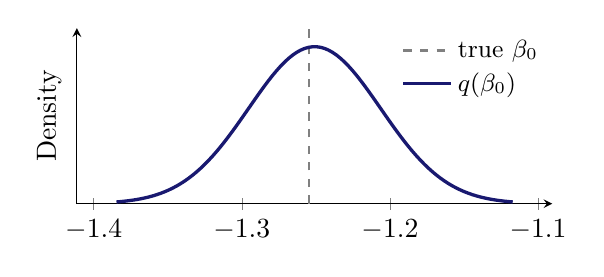
\begin{tikzpicture}

\begin{axis}[
width=3.0in,
height=1.5in,
axis lines=left,
enlarge x limits=0.1,
ylabel={Density},
ylabel near ticks,
ytick=\empty,
legend entries={{true $\beta_0$}, {$q(\beta_0)$}},
legend style={draw=none, at={(1.0,1.0)}, anchor=north east,font=\small},
legend cell align=left,
]
\addplot [thick, dashed, gray]
table {%
-1.25459881152638 0
-1.25459881152638 10
};
\addplot [very thick, MidnightBlue]
table {%
-1.3846001252532 0.0994103432712143
-1.38189822457957 0.119013603277019
-1.37919632390593 0.141960143663186
-1.3764944232323 0.168710087816997
-1.37379252255866 0.199765491467325
-1.37109062188503 0.23567020520197
-1.36838872121139 0.277008877312448
-1.36568682053776 0.324404962879766
-1.36298491986412 0.378517608358809
-1.36028301919048 0.440037289017542
-1.35758111851685 0.509680089993057
-1.35487921784321 0.588180540878532
-1.35217731716958 0.676282938940386
-1.34947541649594 0.774731127379731
-1.34677351582231 0.884256732367532
-1.34407161514867 1.00556590551315
-1.34136971447504 1.1393246663063
-1.3386678138014 1.28614299094489
-1.33596591312777 1.44655784857285
-1.33326401245413 1.62101544176614
-1.3305621117805 1.80985296332854
-1.32786021110686 2.01328023408348
-1.32515831043323 2.23136163420829
-1.32245640975959 2.46399878150339
-1.31975450908596 2.71091444157125
-1.31705260841232 2.97163817504537
-1.31435070773869 3.245494233803
-1.31164880706505 3.53159220986514
-1.30894690639142 3.82882091618547
-1.30624500571778 4.13584593700778
-1.30354310504415 4.45111122675914
-1.30084120437051 4.77284506101201
-1.29813930369688 5.0990705520425
-1.29543740302324 5.42762083676813
-1.29273550234961 5.75615892887182
-1.29003360167597 6.08220210282844
-1.28733170100234 6.40315054899689
-1.2846298003287 6.71631990999255
-1.28192789965507 7.01897718355629
-1.27922599898143 7.30837936054445
-1.2765240983078 7.58181406287413
-1.27382219763416 7.83664135941491
-1.27112029696053 8.07033587163715
-1.26841839628689 8.28052823841812
-1.26571649561326 8.46504499312375
-1.26301459493962 8.62194591739624
-1.26031269426599 8.74955797547933
-1.25761079359235 8.84650499987558
-1.25490889291872 8.91173239208829
-1.25220699224508 8.94452621859864
-1.24950509157145 8.94452621859864
-1.24680319089781 8.91173239208829
-1.24410129022418 8.84650499987558
-1.24139938955054 8.74955797547933
-1.23869748887691 8.62194591739624
-1.23599558820327 8.46504499312375
-1.23329368752964 8.28052823841812
-1.230591786856 8.07033587163715
-1.22788988618237 7.83664135941491
-1.22518798550873 7.58181406287413
-1.2224860848351 7.30837936054445
-1.21978418416146 7.01897718355629
-1.21708228348783 6.71631990999255
-1.21438038281419 6.40315054899689
-1.21167848214056 6.08220210282844
-1.20897658146692 5.75615892887182
-1.20627468079329 5.42762083676813
-1.20357278011965 5.0990705520425
-1.20087087944602 4.77284506101201
-1.19816897877238 4.45111122675914
-1.19546707809875 4.13584593700778
-1.19276517742511 3.82882091618547
-1.19006327675147 3.53159220986514
-1.18736137607784 3.245494233803
-1.1846594754042 2.97163817504537
-1.18195757473057 2.71091444157125
-1.17925567405693 2.46399878150339
-1.1765537733833 2.23136163420829
-1.17385187270966 2.01328023408348
-1.17114997203603 1.80985296332852
-1.16844807136239 1.62101544176614
-1.16574617068876 1.44655784857284
-1.16304427001512 1.28614299094489
-1.16034236934149 1.1393246663063
-1.15764046866785 1.00556590551315
-1.15493856799422 0.884256732367532
-1.15223666732058 0.774731127379731
-1.14953476664695 0.676282938940386
-1.14683286597331 0.588180540878532
-1.14413096529968 0.509680089993057
-1.14142906462604 0.440037289017542
-1.13872716395241 0.378517608358809
-1.13602526327877 0.324404962879766
-1.13332336260514 0.277008877312448
-1.1306214619315 0.23567020520197
-1.12791956125787 0.199765491467325
-1.12521766058423 0.168710087816997
-1.1225157599106 0.141960143663186
-1.11981385923696 0.119013603277019
-1.11711195856333 0.0994103432712143
};
\end{axis}

\end{tikzpicture}

% This file was created by matplotlib2tikz v0.5.15.
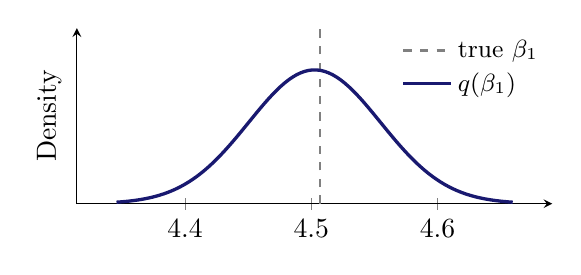
\begin{tikzpicture}

\begin{axis}[
width=3.0in,
height=1.5in,
axis lines=left,
enlarge x limits=0.1,
ylabel={Density},
ylabel near ticks,
ytick=\empty,
legend entries={{true $\beta_1$}, {$q(\beta_1)$}},
legend style={draw=none, at={(1.0,1.0)}, anchor=north east,font=\small},
legend cell align=left,
]
\addplot [thick, dashed, gray]
table {%
4.50714306409916 0
4.50714306409916 10
};
\addplot [very thick, MidnightBlue]
table {%
4.34573828801513 0.0847196368493868
4.34890870851549 0.10142595748068
4.35207912901586 0.120981493700508
4.35524954951622 0.143778372575268
4.35841997001659 0.170244456816511
4.36159039051695 0.200843227615254
4.36476081101732 0.236072934844829
4.36793123151768 0.276464900360839
4.37110165201805 0.32258086297689
4.37427207251841 0.375009260596227
4.37744249301878 0.434360356404465
4.38061291351914 0.501260132350176
4.38378333401951 0.576342894603564
4.38695375451987 0.660242562370592
4.39012417502024 0.753582643240854
4.3932945955206 0.856964934833564
4.39646501602097 0.970957033310708
4.39963543652134 1.0960787735333
4.4028058570217 1.23278777217752
4.40597627752207 1.3814642926944
4.40914669802243 1.5423956980579
4.4123171185228 1.71576080209543
4.41548753902316 1.9016144709815
4.41865795952353 2.09987286128549
4.42182838002389 2.31029970787936
4.42499880052426 2.5324940921969
4.42816922102462 2.7658801271254
4.43133964152499 3.00969898779668
4.43451006202535 3.26300369666362
4.43768048252572 3.52465703586171
4.44085090302608 3.79333290982064
4.44402132352645 4.06752141680225
4.44719174402681 4.34553781048589
4.45036216452718 4.62553544345631
4.45353258502754 4.90552268561157
4.45670300552791 5.18338370475588
4.45987342602827 5.45690288708667
4.46304384652864 5.72379256539229
4.466214267029 5.98172361625076
4.46938468752937 6.22835838815748
4.47255510802973 6.46138533405777
4.4757255285301 6.67855464775127
4.47889594903046 6.8777141472326
4.48206636953083 7.05684461189273
4.48523679003119 7.21409376662747
4.48840721053156 7.34780811554017
4.49157763103192 7.45656186150507
4.49474805153229 7.53918220492418
4.49791847203266 7.59477039423177
4.50108889253302 7.62271799989771
4.50425931303339 7.62271799989771
4.50742973353375 7.59477039423177
4.51060015403412 7.53918220492418
4.51377057453448 7.45656186150507
4.51694099503485 7.34780811554017
4.52011141553521 7.21409376662747
4.52328183603558 7.05684461189273
4.52645225653594 6.8777141472326
4.52962267703631 6.67855464775127
4.53279309753667 6.46138533405777
4.53596351803704 6.22835838815748
4.5391339385374 5.98172361625076
4.54230435903777 5.72379256539229
4.54547477953813 5.45690288708667
4.5486452000385 5.18338370475588
4.55181562053886 4.90552268561157
4.55498604103923 4.62553544345631
4.55815646153959 4.34553781048589
4.56132688203996 4.06752141680225
4.56449730254032 3.79333290982064
4.56766772304069 3.52465703586171
4.57083814354105 3.26300369666362
4.57400856404142 3.00969898779668
4.57717898454178 2.7658801271254
4.58034940504215 2.5324940921969
4.58351982554252 2.31029970787936
4.58669024604288 2.09987286128549
4.58986066654325 1.9016144709815
4.59303108704361 1.71576080209543
4.59620150754398 1.5423956980579
4.59937192804434 1.3814642926944
4.60254234854471 1.23278777217752
4.60571276904507 1.0960787735333
4.60888318954544 0.970957033310708
4.6120536100458 0.856964934833564
4.61522403054617 0.753582643240854
4.61839445104653 0.660242562370592
4.6215648715469 0.576342894603564
4.62473529204726 0.501260132350176
4.62790571254763 0.434360356404465
4.63107613304799 0.375009260596227
4.63424655354836 0.32258086297689
4.63741697404872 0.276464900360839
4.64058739454909 0.236072934844829
4.64375781504945 0.200843227615254
4.64692823554982 0.170244456816511
4.65009865605018 0.143778372575268
4.65326907655055 0.120981493700508
4.65643949705091 0.10142595748068
4.65960991755128 0.0847196368493868
};
\end{axis}

\end{tikzpicture}


\medskip

% This file was created by matplotlib2tikz v0.5.15.
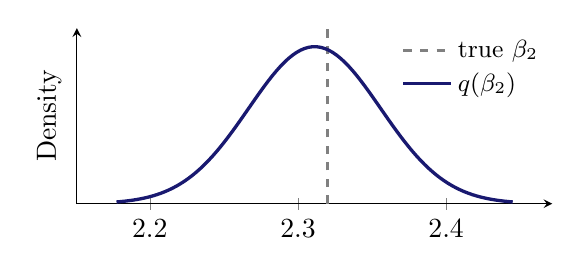
\begin{tikzpicture}

\begin{axis}[
width=3.0in,
height=1.5in,
axis lines=left,
enlarge x limits=0.1,
ylabel={Density},
ylabel near ticks,
ytick=\empty,
legend entries={{true $\beta_2$}, {$q(\beta_2)$}},
legend style={draw=none, at={(1.0,1.0)}, anchor=north east,font=\small},
legend cell align=left,
]
\addplot [thick, dashed, gray]
table {%
2.31993941811405 0
2.31993941811405 10
};
\addplot [very thick, MidnightBlue]
table {%
2.17749552056193 0.0994200051212747
2.18019715865905 0.119025170399235
2.18289879675616 0.141973940996314
2.18560043485327 0.168726485019929
2.18830207295039 0.199784906994549
2.1910037110475 0.235693110365672
2.19370534914461 0.277035800247729
2.19640698724172 0.324436492316309
2.19910862533884 0.378554397089809
2.20181026343595 0.440080056944581
2.20451190153306 0.509729626615162
2.20721353963017 0.588237707084861
2.20991517772729 0.676348667959524
2.2126168158244 0.774806424735553
2.21531845392151 0.884342674691867
2.21802009201863 1.00566363806981
2.22072173011574 1.13943539909057
2.22342336821285 1.28626799323666
2.22612500630996 1.44669844184086
2.22882664440708 1.62117299084632
2.23152828250419 1.8100288658291
2.2342299206013 2.01347590800542
2.23693155869842 2.23157850380988
2.23963319679553 2.46423826148096
2.24233483489264 2.71117791967622
2.24503647298975 2.97192699330649
2.24773811108687 3.24580966857194
2.25043974918398 3.53193545095336
2.25314138728109 3.82919304540647
2.25584302537821 4.13624790648096
2.25854466347532 4.45154383736945
2.26124630157243 4.77330894144763
2.26394793966954 5.09956613885468
2.26664957776666 5.42814835590733
2.26935121586377 5.75671837915301
2.27205285396088 6.0827932417665
2.274754492058 6.40377288142713
2.27745613015511 6.71697267985326
2.28015776825222 7.01965936916085
2.28285940634933 7.3090896736089
2.28556104444645 7.58255095149406
2.28826268254356 7.83740301510686
2.29096432064067 8.07112024047207
2.29366595873779 8.2813330361849
2.2963675968349 8.46586772436868
2.29906923493201 8.62278389809264
2.30177087302912 8.75040835899549
2.30447251112624 8.84736480582791
2.30717414922335 8.91259853759506
2.30987578732046 8.94539555138979
2.31257742541758 8.94539555138979
2.31527906351469 8.91259853759505
2.3179807016118 8.84736480582791
2.32068233970891 8.75040835899549
2.32338397780603 8.62278389809264
2.32608561590314 8.46586772436868
2.32878725400025 8.2813330361849
2.33148889209736 8.07112024047207
2.33419053019448 7.83740301510686
2.33689216829159 7.58255095149406
2.3395938063887 7.3090896736089
2.34229544448582 7.01965936916085
2.34499708258293 6.71697267985321
2.34769872068004 6.40377288142713
2.35040035877715 6.0827932417665
2.35310199687427 5.75671837915301
2.35580363497138 5.42814835590733
2.35850527306849 5.09956613885468
2.36120691116561 4.77330894144763
2.36390854926272 4.45154383736945
2.36661018735983 4.13624790648096
2.36931182545694 3.82919304540647
2.37201346355406 3.53193545095336
2.37471510165117 3.24580966857189
2.37741673974828 2.97192699330649
2.3801183778454 2.71117791967622
2.38282001594251 2.46423826148096
2.38552165403962 2.23157850380988
2.38822329213673 2.01347590800542
2.39092493023385 1.8100288658291
2.39362656833096 1.62117299084632
2.39632820642807 1.44669844184086
2.39902984452519 1.28626799323666
2.4017314826223 1.13943539909057
2.40443312071941 1.00566363806979
2.40713475881652 0.884342674691867
2.40983639691364 0.774806424735553
2.41253803501075 0.676348667959524
2.41523967310786 0.588237707084861
2.41794131120498 0.509729626615162
2.42064294930209 0.440080056944581
2.4233445873992 0.378554397089809
2.42604622549631 0.324436492316309
2.42874786359343 0.277035800247729
2.43144950169054 0.235693110365672
2.43415113978765 0.199784906994543
2.43685277788477 0.168726485019929
2.43955441598188 0.141973940996314
2.44225605407899 0.119025170399235
2.4449576921761 0.0994200051212747
};
\end{axis}

\end{tikzpicture}

% This file was created by matplotlib2tikz v0.5.15.
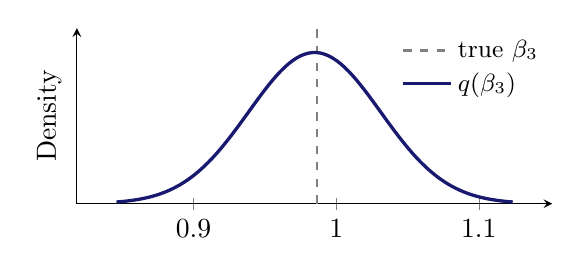
\begin{tikzpicture}

\begin{axis}[
width=3.0in,
height=1.5in,
axis lines=left,
enlarge x limits=0.1,
ylabel={Density},
ylabel near ticks,
ytick=\empty,
legend entries={{true $\beta_3$}, {$q(\beta_3)$}},
legend style={draw=none, at={(1.0,1.0)}, anchor=north east,font=\small},
legend cell align=left,
]
\addplot [thick, dashed, gray]
table {%
0.986584841970366 0
0.986584841970366 10
};
\addplot [very thick, MidnightBlue]
table {%
0.845995739102364 0.0957297390446682
0.848801522092386 0.114607200916625
0.851607305082408 0.136704160356275
0.85441308807243 0.162463704977476
0.857218871062452 0.192369302217613
0.860024654052474 0.226944666945143
0.862830437042496 0.26675280122341
0.865636220032519 0.312394077108754
0.868442003022541 0.364503236581151
0.871247786012563 0.423745190504442
0.874053569002585 0.49080951142261
0.876859351992607 0.566403533441557
0.879665134982629 0.651243996698592
0.882470917972651 0.746047204077195
0.885276700962674 0.851517693758399
0.888082483952696 0.968335472540955
0.890888266942718 1.09714190096996
0.89369404993274 1.23852437126565
0.896499832922762 1.39299997163367
0.899305615912784 1.56099838428567
0.902111398902806 1.74284431767804
0.904917181892829 1.93873982415276
0.907722964882851 2.14874690025235
0.910528747872873 2.37277080631509
0.913334530862895 2.61054457236931
0.916140313852917 2.86161517676441
0.918946096842939 3.12533189051869
0.921751879832961 3.40083727243771
0.924557662822983 3.68706127646313
0.927363445813006 3.98271889272663
0.930169228803028 4.28631168724502
0.93297501179305 4.59613353255179
0.935780794783072 4.91028073392366
0.938586577773094 5.22666665499454
0.941392360763116 5.54304083486749
0.944198143753138 5.85701246933826
0.947003926743161 6.16607800505092
0.949809709733183 6.46765247123206
0.952615492723205 6.75910405327903
0.955421275713227 7.03779130020314
0.958227058703249 7.30110225798107
0.961032841693271 7.54649473724003
0.963838624683293 7.77153685997138
0.966644407673316 7.97394698912894
0.969450190663338 8.15163212928732
0.97225597365336 8.30272389742954
0.975061756643382 8.4256112008756
0.977867539633404 8.5189688238474
0.980673322623426 8.58178121368143
0.983479105613448 8.61336086978972
0.986284888603471 8.61336086978972
0.989090671593493 8.58178121368143
0.991896454583515 8.5189688238474
0.994702237573537 8.4256112008756
0.997508020563559 8.30272389742954
1.00031380355358 8.15163212928732
1.0031195865436 7.97394698912894
1.00592536953363 7.77153685997139
1.00873115252365 7.54649473724004
1.01153693551367 7.30110225798107
1.01434271850369 7.03779130020314
1.01714850149371 6.75910405327903
1.01995428448374 6.46765247123206
1.02276006747376 6.16607800505091
1.02556585046378 5.85701246933825
1.0283716334538 5.54304083486749
1.03117741644382 5.22666665499454
1.03398319943385 4.91028073392366
1.03678898242387 4.5961335325518
1.03959476541389 4.28631168724503
1.04240054840391 3.98271889272663
1.04520633139394 3.68706127646313
1.04801211438396 3.40083727243771
1.05081789737398 3.12533189051869
1.053623680364 2.8616151767644
1.05642946335402 2.6105445723693
1.05923524634405 2.37277080631509
1.06204102933407 2.14874690025235
1.06484681232409 1.93873982415276
1.06765259531411 1.74284431767805
1.07045837830413 1.56099838428568
1.07326416129416 1.39299997163367
1.07606994428418 1.23852437126565
1.0788757272742 1.09714190096996
1.08168151026422 0.96833547254096
1.08448729325425 0.851517693758395
1.08729307624427 0.746047204077192
1.09009885923429 0.651243996698592
1.09290464222431 0.566403533441557
1.09571042521433 0.49080951142261
1.09851620820436 0.423745190504444
1.10132199119438 0.364503236581153
1.1041277741844 0.312394077108753
1.10693355717442 0.26675280122341
1.10973934016444 0.226944666945143
1.11254512315447 0.192369302217614
1.11535090614449 0.162463704977475
1.11815668913451 0.136704160356274
1.12096247212453 0.114607200916625
1.12376825511456 0.0957297390446682
};
\end{axis}

\end{tikzpicture}


\medskip

% This file was created by matplotlib2tikz v0.5.15.
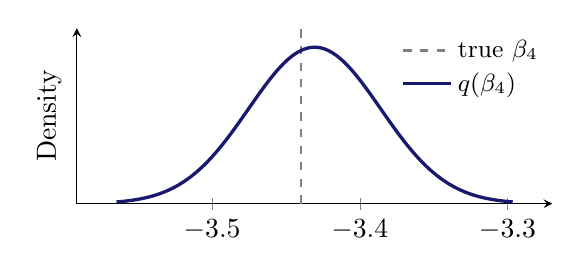
\begin{tikzpicture}

\begin{axis}[
width=3.0in,
height=1.5in,
axis lines=left,
enlarge x limits=0.1,
ylabel={Density},
ylabel near ticks,
ytick=\empty,
legend entries={{true $\beta_4$}, {$q(\beta_4)$}},
legend style={draw=none, at={(1.0,1.0)}, anchor=north east,font=\small},
legend cell align=left,
]
\addplot [thick, dashed, gray]
table {%
-3.43981359557564 0
-3.43981359557564 10
};
\addplot [very thick, MidnightBlue]
table {%
-3.56477700546384 0.0990877818607054
-3.56206630926692 0.118627434247927
-3.55935561307 0.141499518916615
-3.55664491687309 0.168162666270076
-3.55393422067617 0.199117302993386
-3.55122352447925 0.234905515016792
-3.54851282828233 0.276110053596034
-3.54580213208542 0.323352350858125
-3.5430914358885 0.3772894144945
-3.54038073969158 0.43860947935558
-3.53767004349467 0.508026307063375
-3.53495934729775 0.586272043848377
-3.53224865110083 0.674088571920725
-3.52953795490391 0.772217320898544
-3.526827258707 0.881387543010997
-3.52411656251008 1.00230309858413
-3.52140586631316 1.13562784604295
-3.51869517011624 1.28196978236695
-3.51598447391933 1.44186413437105
-3.51327377772241 1.61575565681672
-3.51056308152549 1.80398044840246
-3.50785238532857 2.00674764913621
-3.50514168913166 2.2241214302979
-3.50243099293474 2.45600372891326
-3.49972029673782 2.70211821014031
-3.49700960054091 2.96199596106921
-3.49429890434399 3.23496342620889
-3.49158820814707 3.52013308672892
-3.48887751195015 3.81639736110385
-3.48616681575324 4.12242616341894
-3.48345611955632 4.43666849707539
-3.4807454233594 4.75735838644311
-3.47803472716248 5.08252535829877
-3.47532403096557 5.41000958048226
-3.47261333476865 5.73748164960578
-3.46990263857173 6.06246689596034
-3.46719194237481 6.38237394562925
-3.4644812461779 6.6945271512885
-3.46177054998098 6.99620237857971
-3.45905985378406 7.28466551872985
-3.45634915758715 7.55721299463653
-3.45363846139023 7.81121344107799
-3.45092776519331 8.04414967373889
-3.44821706899639 8.2536600194738
-3.44550637279948 8.43757806399793
-3.44279567660256 8.59396988447118
-3.44008498040564 8.72116787371497
-3.43737428420872 8.81780032954718
-3.43466358801181 8.88281607537638
-3.43195289181489 8.9155034942174
-3.42924219561797 8.9155034942174
-3.42653149942105 8.88281607537638
-3.42382080322414 8.81780032954718
-3.42111010702722 8.72116787371497
-3.4183994108303 8.59396988447118
-3.41568871463339 8.43757806399793
-3.41297801843647 8.2536600194738
-3.41026732223955 8.04414967373889
-3.40755662604263 7.81121344107799
-3.40484592984572 7.55721299463653
-3.4021352336488 7.2846655187298
-3.39942453745188 6.99620237857971
-3.39671384125496 6.6945271512885
-3.39400314505805 6.38237394562925
-3.39129244886113 6.06246689596034
-3.38858175266421 5.73748164960578
-3.38587105646729 5.41000958048226
-3.38316036027038 5.08252535829877
-3.38044966407346 4.75735838644311
-3.37773896787654 4.43666849707539
-3.37502827167963 4.12242616341894
-3.37231757548271 3.81639736110385
-3.36960687928579 3.52013308672892
-3.36689618308887 3.23496342620889
-3.36418548689196 2.96199596106921
-3.36147479069504 2.70211821014031
-3.35876409449812 2.45600372891326
-3.3560533983012 2.2241214302979
-3.35334270210429 2.00674764913621
-3.35063200590737 1.80398044840246
-3.34792130971045 1.61575565681672
-3.34521061351353 1.44186413437105
-3.34249991731662 1.28196978236695
-3.3397892211197 1.13562784604295
-3.33707852492278 1.00230309858413
-3.33436782872587 0.881387543010997
-3.33165713252895 0.772217320898544
-3.32894643633203 0.674088571920725
-3.32623574013511 0.586272043848377
-3.3235250439382 0.508026307063375
-3.32081434774128 0.43860947935558
-3.31810365154436 0.3772894144945
-3.31539295534744 0.323352350858125
-3.31268225915053 0.276110053596027
-3.30997156295361 0.234905515016792
-3.30726086675669 0.199117302993386
-3.30455017055977 0.168162666270076
-3.30183947436286 0.141499518916615
-3.29912877816594 0.118627434247927
-3.29641808196902 0.0990877818607054
};
\end{axis}

\end{tikzpicture}

\caption{Visualization of the inferred marginal posteriors for Bayesian linear
regression. The gray bars indicate the simulated ``true'' value for each
component of the coefficient vector.}
\label{fig:supervised-betas}
\end{figure}

\subsubsection{Criticism}

A standard evaluation in regression is to calculate point-based evaluations on
held-out ``testing'' data. We do this first by forming the posterior predictive
distribution.
\begin{lstlisting}
y_post = Normal(mu=ed.dot(X, qw.mean()) + qb.mean(), sigma=tf.ones(N))
\end{lstlisting}

With this we can evaluate various point-based quantities using the posterior
predictive.
\begin{lstlisting}
print(ed.evaluate('mean_squared_error', data={X: X_test, y_post: y_test}))
> 0.012107

print(ed.evaluate('mean_absolute_error', data={X: X_test, y_post: y_test}))
> 0.0867875
\end{lstlisting}

The trained model makes predictions with low mean squared error
(relative to the magnitude of the output).

Edward supports another class of criticism techniques called
\glspl{PPC}.
The simplest \gls{PPC} works by applying a test statistic on new data
generated from the posterior predictive, such as
$T(\mathbf{x}_\text{new}) = \max(\mathbf{x}_\text{new})$.
Applying $T(\mathbf{x}_\text{new})$ to
new data over many data replications induces a distribution of the test
statistic, $\textsc{ppd}(T)$. We compare
this distribution to the test statistic applied to the original dataset
$T(\mathbf{x})$.

Calculating \glspl{PPC} in Edward is straightforward.
\begin{lstlisting}
def T(xs, zs):
  return tf.reduce_max(xs[y_post])

ppc_max = ed.ppc(T, data={X: X_train, y_post: y_train})
\end{lstlisting}
This calculates the test statistic on both the original dataset as well as on
data replications generated from teh posterior predictive distribution.
Figure \ref{fig:supervised-ppc} shows three visualizations of different \glspl
{PPC}; the
plotted posterior predictive distributions are kernel density estimates from
$N=500$ data replications.


\begin{figure}[htb]
\centering
% This file was created by matplotlib2tikz v0.5.15.
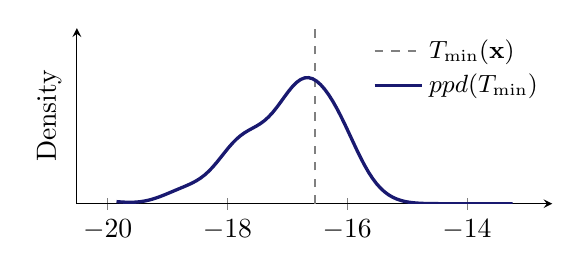
\begin{tikzpicture}

\begin{axis}[
width=3.0in,
height=1.5in,
axis lines=left,
enlarge x limits=0.1,
ylabel={Density},
ylabel near ticks,
ytick=\empty,
legend entries={{$T_\text{min}(\mathbf{x})$}, {$\textsc{ppd}(T_\text{min})$}},
legend style={draw=none, at={(1.0,1.0)}, anchor=north east,font=\small},
legend cell align=left,
]
\addplot [thick, dashed, gray]
table {%
-16.5441242364738 0
-16.5441242364738 0.7
};
\addplot [very thick, MidnightBlue]
table {%
-13.2352993891791 5.05219293070858e-13
-13.3021443355891 2.05825068882034e-12
-13.3689892819991 8.038769482291e-12
-13.4358342284091 3.01002711420105e-11
-13.5026791748191 1.08058842088904e-10
-13.5695241212291 3.71948112238135e-10
-13.6363690676391 1.22761967091541e-09
-13.703214014049 3.88541167689218e-09
-13.770058960459 1.17934327544065e-08
-13.836903906869 3.43335601433984e-08
-13.903748853279 9.58797378067529e-08
-13.970593799689 2.56878942376166e-07
-14.037438746099 6.60390007322067e-07
-14.104283692509 1.62942503466722e-06
-14.171128638919 3.85957766174606e-06
-14.237973585329 8.77906132307628e-06
-14.304818531739 1.91830211203899e-05
-14.371663478149 4.02843232474005e-05
-14.438508424559 8.13454163652436e-05
-14.505353370969 0.000158045340654349
-14.572198317379 0.000295671862401375
-14.639043263789 0.000533101503267019
-14.705888210199 0.000927356629459576
-14.772733156609 0.00155836143375224
-14.839578103019 0.0025334377221303
-14.906423049429 0.00399115809416706
-14.973267995839 0.00610441074410488
-15.040112942249 0.00908280448773802
-15.1069578886589 0.0131746032563921
-15.1738028350689 0.0186679352142648
-15.2406477814789 0.0258899291011952
-15.3074927278889 0.0352009076844701
-15.3743376742989 0.0469795037322437
-15.4411826207089 0.061594575989866
-15.5080275671189 0.0793620014551975
-15.5748725135289 0.100488999535781
-15.6417174599389 0.125014606287185
-15.7085624063489 0.152760090791724
-15.7754073527589 0.183304841215112
-15.8422522991689 0.215999631691617
-15.9090972455789 0.250020225923821
-15.9759421919889 0.284452402130418
-16.0427871383989 0.318388874103353
-16.1096320848089 0.351013519104097
-16.1764770312189 0.38165129488892
-16.2433219776289 0.409772728951764
-16.3101669240389 0.434956507091933
-16.3770118704489 0.456827556412376
-16.4438568168589 0.474996523312243
-16.5107017632689 0.489026959953148
-16.5775467096788 0.498448653141407
-16.6443916560888 0.502821529311249
-16.7112366024988 0.501838316951246
-16.7780815489088 0.495440274532375
-16.8449264953188 0.483913062864297
-16.9117714417288 0.467931894223707
-16.9786163881388 0.448536362773748
-17.0454613345488 0.427032755011925
-17.1123062809588 0.404839873801779
-17.1791512273688 0.383307916393971
-17.2459961737788 0.363545023299929
-17.3128411201888 0.346282271150708
-17.3796860665988 0.331797694426288
-17.4465310130088 0.319907513582849
-17.5133759594188 0.31002177463391
-17.5802209058288 0.301253806284686
-17.6470658522388 0.292567919168833
-17.7139107986488 0.282946187091122
-17.7807557450588 0.271552000520565
-17.8476006914688 0.257865922265467
-17.9144456378788 0.241770195825571
-17.9812905842888 0.223564258665736
-18.0481355306987 0.20390550471423
-18.1149804771087 0.183685389894948
-18.1818254235187 0.163866398952204
-18.2486703699287 0.145315174953473
-18.3155153163387 0.128667506515823
-18.3823602627487 0.114251399827959
-18.4492052091587 0.102078285357883
-18.5160501555687 0.0918949883808782
-18.5828951019787 0.0832759071210482
-18.6497400483887 0.0757292467898767
-18.7165849947987 0.0687933906826522
-18.7834299412087 0.0621071419943456
-18.8502748876187 0.0554470682033875
-18.9171198340287 0.0487334112562898
-18.9839647804387 0.0420113379764541
-19.0508097268487 0.0354165758884345
-19.1176546732587 0.0291345116183055
-19.1844996196687 0.023360572096513
-19.2513445660787 0.0182677812430854
-19.3181895124887 0.0139850418440157
-19.3850344588987 0.0105870889772692
-19.4518794053086 0.00809451956674418
-19.5187243517186 0.0064803640817207
-19.5855692981286 0.0056788992121118
-19.6524142445386 0.00559309392058319
-19.7192591909486 0.00609902076360903
-19.7861041373586 0.00704802346396004
-19.8529490837686 0.00826940904339173
};
\end{axis}

\end{tikzpicture}

% This file was created by matplotlib2tikz v0.5.15.
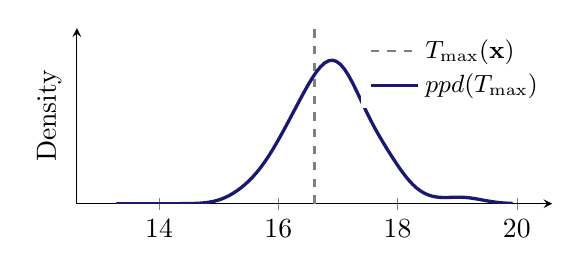
\begin{tikzpicture}

\begin{axis}[
width=3.0in,
height=1.5in,
axis lines=left,
enlarge x limits=0.1,
ylabel={Density},
ylabel near ticks,
ytick=\empty,
legend entries={{$T_\text{max}(\mathbf{x})$}, {$\textsc{ppd}(T_\text{max})$}},
legend style={draw=none, at={(1.0,1.0)}, anchor=north east,font=\small},
legend cell align=left,
]
\addplot [thick, dashed, gray]
table {%
16.6090179263646 0
16.6090179263646 0.7
};
\addplot [very thick, MidnightBlue]
table {%
13.2872143410917 5.88907908239748e-12
13.3543214842285 2.30682665294251e-11
13.4214286273653 8.65546789880128e-11
13.4885357705022 3.1109455968171e-10
13.555642913639 1.0711268332124e-09
13.6227500567758 3.53312245190288e-09
13.6898571999126 1.11653193225071e-08
13.7569643430495 3.3807003201652e-08
13.8240714861863 9.80837688954409e-08
13.8911786293231 2.72695790757017e-07
13.9582857724599 7.26592725735176e-07
14.0253929155968 1.85558514831365e-06
14.0925000587336 4.54255547295968e-06
14.1596072018704 1.06612705924626e-05
14.2267143450072 2.39925316082358e-05
14.2938214881441 5.17823461453552e-05
14.3609286312809 0.0001072061804853
14.4280357744177 0.000212961676966936
14.4951429175546 0.000406031146985154
14.5622500606914 0.000743282168077874
14.6293572038282 0.00130701292524395
14.696464346965 0.0022089106794077
14.7635714901019 0.00359042894948312
14.8306786332387 0.00561765895060876
14.8977857763755 0.00846970343296913
14.9648929195123 0.0123214421175529
15.0320000626492 0.0173240355812697
15.099107205786 0.0235886564903373
15.1662143489228 0.031179576611542
15.2333214920596 0.0401209248561671
15.3004286351965 0.0504171026374971
15.3675357783333 0.0620812265945392
15.4346429214701 0.0751613769177472
15.501750064607 0.0897533274782765
15.5688572077438 0.105992124712952
15.6359643508806 0.124022507817905
15.7030714940174 0.143956727359728
15.7701786371543 0.165833949246076
15.8372857802911 0.189595328748755
15.9043929234279 0.215082843128724
15.9715000665647 0.242060737082459
16.0386072097016 0.270250050733925
16.1057143528384 0.299362541219018
16.1728214959752 0.32912144615983
16.239928639112 0.359261610668238
16.3070357822489 0.389507960577613
16.3741429253857 0.419537018754109
16.4412500685225 0.448930257716725
16.5083572116594 0.477130658103593
16.5754643547962 0.503415058089259
16.642571497933 0.526894349720654
16.7096786410698 0.546550574825499
16.7767857842067 0.561314151873328
16.8438929273435 0.570176434087392
16.9110000704803 0.572324061977174
16.9781072136171 0.567274001154524
17.045214356754 0.554983501388671
17.1123214998908 0.535908974244704
17.1794286430276 0.51099320138505
17.2465357861644 0.481571955357454
17.3136429293013 0.449208111466936
17.3807500724381 0.415480326874349
17.4478572155749 0.381768753084954
17.5149643587118 0.349085826732023
17.5820715018486 0.317991959931194
17.6491786449854 0.28861464804705
17.7162857881222 0.260761178662522
17.7833929312591 0.234089181792312
17.8505000743959 0.208284730263077
17.9176072175327 0.183199427299166
17.9847143606695 0.15891462704636
18.0518215038064 0.135725953354043
18.1189286469432 0.114065475069874
18.18603579008 0.0943943177157276
18.2531429332168 0.0771011977617766
18.3202500763537 0.062433366545238
18.3873572194905 0.0504707003030209
18.4544643626273 0.0411377501446338
18.5215715057642 0.0342380739875309
18.588678648901 0.0294928336595045
18.6557857920378 0.0265706969754408
18.7228929351746 0.025105076939142
18.7900000783115 0.0247032169000523
18.8571072214483 0.0249560346592097
18.9242143645851 0.0254566143186622
18.9913215077219 0.0258298999634965
19.0584286508588 0.0257693361585591
19.1255357939956 0.0250711059829185
19.1926429371324 0.0236554243582867
19.2597500802692 0.0215674372259132
19.3268572234061 0.0189562594568207
19.3939643665429 0.0160371232920431
19.4610715096797 0.0130461174367693
19.5281786528165 0.0101981696569966
19.5952857959534 0.00765675999972511
19.6623929390902 0.00551954424981433
19.729500082227 0.0038193648300069
19.7966072253639 0.00253657419000109
19.8637143685007 0.00161701386050297
19.9308215116375 0.000990349592964849
};
\end{axis}

\end{tikzpicture}


\medskip

% This file was created by matplotlib2tikz v0.5.15.
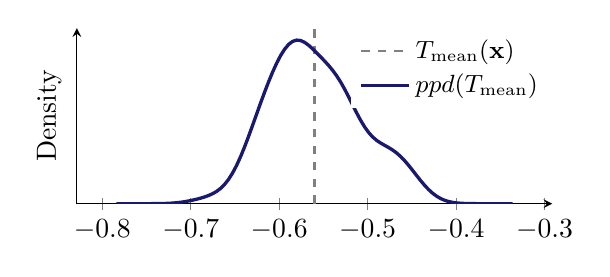
\begin{tikzpicture}

\begin{axis}[
width=3.0in,
height=1.5in,
axis lines=left,
enlarge x limits=0.1,
ylabel={Density},
ylabel near ticks,
ytick=\empty,
legend entries={{$T_\text{mean}(\mathbf{x})$}, {$\textsc{ppd}(T_\text{mean})$}},
legend style={draw=none, at={(1.0,1.0)}, anchor=north east,font=\small},
legend cell align=left,
]
\addplot [thick, dashed, gray]
table {%
-0.559917133751622 0
-0.559917133751622 8
};
\addplot [very thick, MidnightBlue]
table {%
-0.335950280250973 1.31826193247141e-07
-0.340474863149976 4.40417152547664e-07
-0.344999446048979 1.40051041254e-06
-0.349524028947982 4.23967782308379e-06
-0.354048611846985 1.22201874775514e-05
-0.358573194745988 3.3543340518437e-05
-0.363097777644991 8.77032514473706e-05
-0.367622360543994 0.000218483251802879
-0.372146943442997 0.000518731692386615
-0.376671526342 0.0011741899396429
-0.381196109241003 0.00253499069727522
-0.385720692140006 0.00522221230327025
-0.390245275039009 0.0102707121664167
-0.394769857938012 0.019296407749699
-0.399294440837015 0.0346563621203797
-0.403819023736018 0.0595475810788749
-0.408343606635021 0.097974212874276
-0.412868189534024 0.154514642298559
-0.417392772433027 0.233849438781403
-0.42191735533203 0.34006905738358
-0.426441938231033 0.475853928256519
-0.430966521130036 0.641684585993456
-0.435491104029039 0.835268781763808
-0.440015686928042 1.05135004425149
-0.444540269827045 1.28199255463699
-0.449064852726048 1.51734460173359
-0.453589435625051 1.74679787721112
-0.458114018524054 1.96040229159795
-0.462638601423057 2.15036528409097
-0.46716318432206 2.31244527582332
-0.471687767221063 2.4470278702521
-0.476212350120066 2.55965637579346
-0.480736933019069 2.66080216636917
-0.485261515918072 2.76473802573947
-0.489786098817075 2.88753333272035
-0.494310681716078 3.04440269712009
-0.498835264615081 3.24685395853415
-0.503359847514084 3.50022588193761
-0.507884430413087 3.80221894074062
-0.51240901331209 4.14287445862823
-0.516933596211093 4.5061614945854
-0.521458179110096 4.87294490313373
-0.525982762009099 5.22472548384073
-0.530507344908102 5.54727438361957
-0.535031927807105 5.83322641691359
-0.539556510706108 6.08290049624787
-0.544081093605111 6.30305460135884
-0.548605676504114 6.50385157623385
-0.553130259403117 6.69484690038952
-0.55765484230212 6.88113690254679
-0.562179425201123 7.06080036809693
-0.566704008100126 7.22440154665388
-0.571228590999129 7.35669463994601
-0.575753173898132 7.43998095855344
-0.580277756797135 7.4580631623682
-0.584802339696138 7.39960494788908
-0.589326922595141 7.25998696678778
-0.593851505494144 7.04132844890974
-0.598376088393147 6.75097937727867
-0.60290067129215 6.39923484102435
-0.607425254191153 5.99714012155065
-0.611949837090156 5.55505271572972
-0.616474419989159 5.08223599892622
-0.620999002888162 4.58734843736424
-0.625523585787165 4.07939787597822
-0.630048168686168 3.56862012110047
-0.634572751585171 3.06681792580805
-0.639097334484174 2.58691662728942
-0.643621917383177 2.14178028998728
-0.64814650028218 1.74259488341976
-0.652671083181183 1.39727785944853
-0.657195666080186 1.10936936894104
-0.661720248979189 0.87770989538598
-0.666244831878192 0.696974855475188
-0.670769414777195 0.558903275250046
-0.675293997676198 0.453895730432368
-0.679818580575201 0.372601409041363
-0.684343163474204 0.307163343307327
-0.688867746373207 0.251916462815002
-0.69339232927221 0.203493603930414
-0.697916912171213 0.160444778103095
-0.702441495070216 0.12257535509535
-0.706966077969219 0.0902362521484529
-0.711490660868222 0.0637553138982275
-0.716015243767225 0.0431095405530541
-0.720539826666228 0.0278410195212284
-0.725064409565231 0.0171492513326823
-0.729588992464234 0.0100653399100707
-0.734113575363237 0.00562517074090984
-0.73863815826224 0.00299195464813669
-0.743162741161243 0.00151403282434576
-0.747687324060246 0.000728732711755793
-0.752211906959249 0.000333561443670076
-0.756736489858252 0.000145178214655598
-0.761261072757255 6.00764012086311e-05
-0.765785655656258 2.363486586849e-05
-0.770310238555261 8.83948805819745e-06
-0.774834821454264 3.14274855194534e-06
-0.779359404353267 1.0621571788719e-06
-0.78388398725227 3.41236740996593e-07
};
\end{axis}

\end{tikzpicture}

\glsreset{PPC}
\caption{Examples of \glspl{PPC} for Bayesian linear regression. }
\label{fig:supervised-ppc}
\end{figure}





\subsection{Logistic and Neural Network Classification}

In supervised learning, the task is to infer hidden structure from
labeled data, comprised of training examples $\{(x_n, y_n)\}$.
Classification means the output $y$ takes discrete values.


\subsubsection{Data}

We study a two-dimensional simulated dataset with a nonlinear decision
boundary. We simulate $100$ datapoints using the following snippet.
\begin{lstlisting}
from scipy.stats import logistic

N = 100  # number of data points
D = 2  # number of features

px1 = np.linspace(-3, 3, 50)
px2 = np.linspace(-3, 3, 50)
px1_m, px2_m = np.mgrid[-3:3:50j, -3:3:50j]

xeval = np.vstack((px1_m.flatten(), px2_m.flatten())).T
x_viz = tf.constant(np.array(xeval, dtype='float32'))

def build_toy_dataset(N):
  x = xeval[np.random.randint(xeval.shape[0],size=N), :]
  y = bernoulli.rvs(p=logistic.cdf( 5 * x[:, 0]**2 + 5 * x[:, 1]**3 ))
  return x, y

x_train, y_train = build_toy_dataset(N)
\end{lstlisting}

Figure\nobreakspace \ref{fig:lr_data} shows the data, colored by label. The red point near the
origin makes this a challenging dataset for classification models that assume a
linear decision boundary.
\begin{figure}[!htbp]
\centering
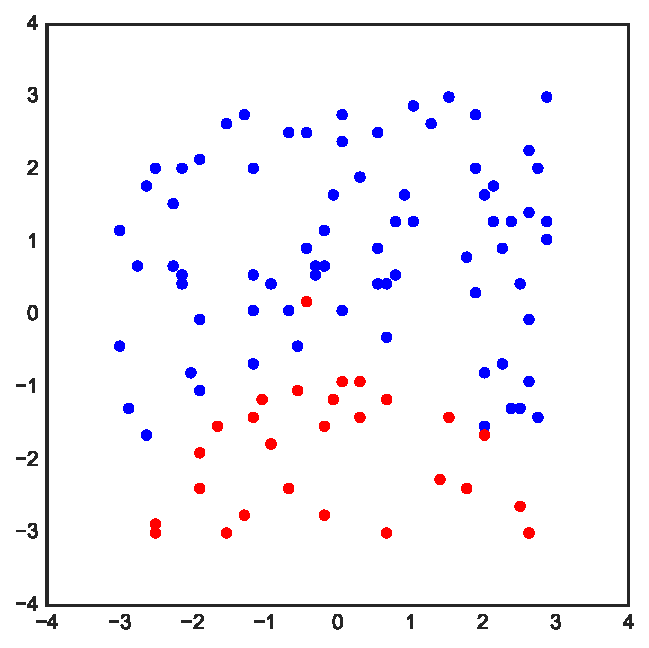
\includegraphics[width=2.5in]{images/lr_data.pdf}
\caption{Simulated data for classification. Positive and negative measurements
colored by label.}
\label{fig:lr_data}
\end{figure}


\subsubsection{Model: Bayesian Logistic Regression}

We begin with a popular classification model: logistic regression. This model
relates outputs $y\in\{0,1\}$, also known as the response, given
a vector of inputs $\mathbf{x}\in\mathbb{R}^D$, also known as the features or
covariates. The model assumes a latent linear relationship between these two random
variables \citep{gelman2013bayesian}.

The likelihood of each datapoint is a Bernoulli with probability
\begin{align*}
\Pr(y_n=1)
  &=
  \text{logistic}
  \left(
  \mathbf{x}^\top \mathbf{w} + b
  \right).
\end{align*}
We posit priors on the latent variables $\mathbf{w}$ and $b$ as
\begin{align*}
  p(\mathbf{w})
  &=
  \text{Normal}(\mathbf{w} \mid \mathbf{0}, \sigma_w^2\mathbf{I}),
  \\
  p(b)
  &=
  \text{Normal}(b \mid 0, \sigma_b^2).
\end{align*}

This model is
easy to specify in Edward's native language.

\begin{lstlisting}
W = Normal(mu=tf.zeros(D), sigma=tf.ones(D))
b = Normal(mu=tf.zeros(1), sigma=tf.ones(1))

x = tf.cast(x_train, dtype=tf.float32)
y = Bernoulli(logits=(ed.dot(x, W) + b))
\end{lstlisting}


\subsubsection{Inference}

Here, we perform variational inference. Define the variational model to be a
fully factorized normal
\begin{lstlisting}
qW = Normal(mu=tf.Variable(tf.random_normal([D])),
            sigma=tf.nn.softplus(tf.Variable(tf.random_normal([D]))))
qb = Normal(mu=tf.Variable(tf.random_normal([1])),
            sigma=tf.nn.softplus(tf.Variable(tf.random_normal([1]))))
\end{lstlisting}

Run variational inference with the Kullback-Leibler divergence for $1000$ iterations.
\begin{lstlisting}
inference = ed.KLqp({W: qW, b: qb}, data={y: y_train})
inference.run(n_iter=1000, n_print=100, n_samples=5)
\end{lstlisting}
In this case
\texttt{KLqp} defaults to minimizing the
$\text{KL}(q\|p)$ divergence measure using the reparameterization
gradient.


\subsubsection{Criticism}

The first thing to look at are point-wise evaluations on the training dataset.

First form a plug-in estimate of the posterior predictive distribution.
\begin{lstlisting}
y_post = ed.copy(y, {W: qW.mean(), b: qb.mean()})
\end{lstlisting}

Then evaluate predictive accuracy
\begin{lstlisting}
print('Plugin estimate of posterior predictive log accuracy on training data:')
print(ed.evaluate('log_lik', data={x: x_train, y_post: y_train}))
> -3.12

print('Binary accuracy on training data:')
print(ed.evaluate('binary_accuracy', data={x: x_train, y_post: y_train}))
> 0.71
\end{lstlisting}

Figure\nobreakspace \ref {fig:lr_linear} shows the posterior label probability evaluated on a grid.
As expected, logistic regression attempts to fit a linear boundary between the
two label classes. Can a non-linear model do better?
\begin{figure}[!htb]
\centering
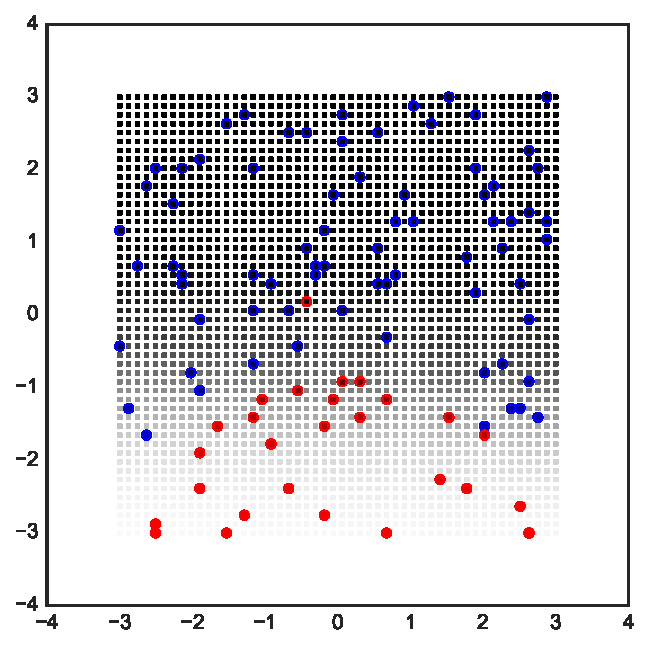
\includegraphics[width=2.5in]{images/lr_linear.pdf}
\caption{Logistic regression struggles to separate the measurements.}
\label{fig:lr_linear}
\end{figure}

\subsubsection{Model: Bayesian Neural Network Classification}

Consider parameterizing the label probability using a neural network; this
model is not limited to a linear relationship to the inputs $\mathbf{x}$, as in
logistic regression.

The model posits a likelihood for each observation $(\mathbf{x}_n,
y_n)$ as
\begin{align*}
\Pr(y_n=1)
  &=
  \text{logistic}
  \left(
  \text{NN}(\mathbf{x}_n \;;\; \mathbf{z})
  \right),
\end{align*}
where NN is a neural network and the latent random variable $\mathbf{z}$
contains its weights and biases.

We can specify a Bayesian neural network in Edward as follows. Here we specify a
fully connected two-layer network with two nodes in each layer; we posit
standard normal priors on all weights and biases.
\begin{lstlisting}
def neural_network(x, W_0, W_1, W_2, b_0, b_1, b_2):
    h = tf.nn.tanh(tf.matmul(x, W_0) + b_0)
    h = tf.nn.tanh(tf.matmul(h, W_1) + b_1)
    h = tf.matmul(h, W_2) + b_2
    return tf.reshape(h, [-1])

H = 2  # number of hidden units in each layer

W_0 = Normal(mu=tf.zeros([D, H]), sigma=tf.ones([D, H]))
W_1 = Normal(mu=tf.zeros([H, H]), sigma=tf.ones([H, H]))
W_2 = Normal(mu=tf.zeros([H, 1]), sigma=tf.ones([H, 1]))
b_0 = Normal(mu=tf.zeros(H), sigma=tf.ones(H))
b_1 = Normal(mu=tf.zeros(H), sigma=tf.ones(H))
b_2 = Normal(mu=tf.zeros(1), sigma=tf.ones(1))

x = tf.cast(x_train, dtype=tf.float32)
y = Bernoulli(logits=neural_network(x, W_0, W_1, W_2, b_0, b_1, b_2))
\end{lstlisting}

\subsubsection{Inference}

Similar to the above, we perform variational inference. Define the variational
model to be a fully factorized normal over all latent variables
\begin{lstlisting}
qW_0 = Normal(mu=tf.Variable(tf.random_normal([D, H])),
              sigma=tf.nn.softplus(tf.Variable(tf.random_normal([D, H]))))
qW_1 = Normal(mu=tf.Variable(tf.random_normal([H, H])),
              sigma=tf.nn.softplus(tf.Variable(tf.random_normal([H, H]))))
qW_2 = Normal(mu=tf.Variable(tf.random_normal([H, 1])),
              sigma=tf.nn.softplus(tf.Variable(tf.random_normal([H, 1]))))
qb_0 = Normal(mu=tf.Variable(tf.random_normal([H])),
              sigma=tf.nn.softplus(tf.Variable(tf.random_normal([H]))))
qb_1 = Normal(mu=tf.Variable(tf.random_normal([H])),
              sigma=tf.nn.softplus(tf.Variable(tf.random_normal([H]))))
qb_2 = Normal(mu=tf.Variable(tf.random_normal([1])),
              sigma=tf.nn.softplus(tf.Variable(tf.random_normal([1]))))
\end{lstlisting}

Run variational inference for $1000$ iterations.
\begin{lstlisting}
inference = ed.KLqp({W_0: qW_0, b_0: qb_0,
                     W_1: qW_1, b_1: qb_1,
                     W_2: qW_2, b_2: qb_2}, data={y: y_train})
inference.run(n_iter=1000, n_print=100, n_samples=5)
\end{lstlisting}

\subsubsection{Criticism}

Again, we form a plug-in estimate of the posterior predictive distribution.
\begin{lstlisting}
y_post = ed.copy(y, {W_0: qW_0.mean(), b_0: qb_0.mean(),
                     W_1: qW_1.mean(), b_1: qb_1.mean(),
                     W_2: qW_2.mean(), b_1: qb_2.mean()})
\end{lstlisting}

Both predictive accuracy metrics look better.
\begin{lstlisting}
print('Plugin estimate of posterior predictive log accuracy on training data:')
print(ed.evaluate('log_lik', data={x: x_train, y_post: y_train}))
> -0.170941

print('Binary accuracy on training data:')
print(ed.evaluate('binary_accuracy', data={x: x_train, y_post: y_train}))
> 0.81
\end{lstlisting}

Figure\nobreakspace \ref{fig:lr_nn} shows the posterior label probability evaluated on a grid.
The neural network has captured the nonlinear decision boundary between the two
label classes.
\begin{figure}[!htb]
\centering
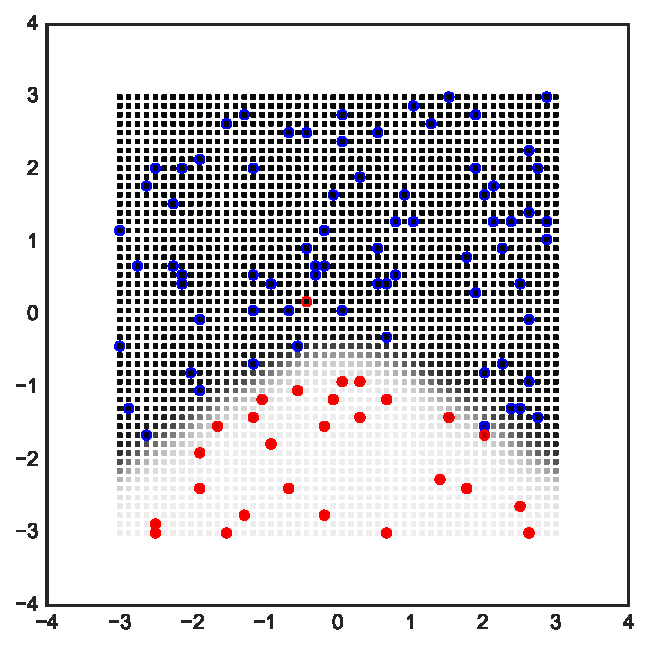
\includegraphics[width=2.5in]{images/lr_nn.pdf}
\caption{A Bayesian neural network does a better job of separating the two
label classes.}
\label{fig:lr_nn}
\end{figure}


\clearpage
\section{Acknowledgments}
Edward has benefited enormously from the helpful feedback and advice
of many individuals: Jaan Altosaar, Eugene Brevdo, Allison Chaney,
Joshua Dillon, Matthew Hoffman, Kevin Murphy, Rajesh Ranganath, Rif
Saurous, and other members of the Blei Lab, Google Brain, and Google
Research.
This work is supported by NSF IIS-1247664, ONR N00014-11-1-0651,
DARPA FA8750-14-2-0009, DARPA N66001-15-C-4032, Adobe, Google, NSERC
PGS-D, and the Sloan Foundation.

\clearpage
\bibliographystyle{apalike}
\bibliography{bib}

\end{document}
